\documentclass[12pt,a4paper]{report}
\usepackage{lipsum}% http://ctan.org/pkg/lipsum
\usepackage{titletoc}% http://ctan.org/pkg/titletoc
\usepackage[T1]{fontenc}
\usepackage{natbib}
\usepackage{url}
\usepackage{titlesec}
\usepackage{graphicx}
\usepackage{subfig}
\usepackage{array}% http://ctan.org/pkg/array
\usepackage{placeins}
\usepackage{amsmath,amssymb}
\usepackage{booktabs, makecell}
\usepackage{siunitx, mhchem}
\usepackage{enumitem}
\usepackage{adjustbox}
\usepackage[ruled,longend]{algorithm2e}

\usepackage{layout}
\setlength{\voffset}{-0.5in}
\setlength{\headsep}{5pt}
\def\x#1{\texttt{\expandafter\string\csname#1\endcsname}&\expandafter$\csname#1\endcsname$}

\newenvironment{tightcenter}{%
  \setlength\topsep{0pt}
  \setlength\parskip{0pt}
  \begin{center}
}{%
  \end{center}
}

\usepackage{hyperref}
\hypersetup{
    colorlinks,
    citecolor=black,
    filecolor=black,
    linkcolor=black,
    urlcolor=black
}

\usepackage{float}
\graphicspath{ {images/} }
\tolerance=1
\emergencystretch=\maxdimen
\hyphenpenalty=10000
\hbadness=10000  
\titleformat{\chapter}{\normalfont\huge}{\thechapter.}{20pt}{\huge}
\titlespacing*{\chapter}{0pt}{0pt}{20pt}

\usepackage{xcolor}
\usepackage{listings}
\usepackage{color}
\definecolor{lightgray}{rgb}{.9,.9,.9}
\definecolor{darkgray}{rgb}{.4,.4,.4}
\definecolor{purple}{rgb}{0.65, 0.12, 0.82}
\definecolor{background}{HTML}{EEEEEE}
\lstdefinelanguage{JavaScript}{
  keywords={break, case, catch, continue, debugger, default, delete, do, else, false, finally, for, function, if, in, instanceof, new, null, return, switch, this, throw, true, try, typeof, var, void, while, with},
  morecomment=[l]{//},
  morecomment=[s]{/*}{*/},
  morestring=[b]',
  morestring=[b]",
  ndkeywords={class, export, boolean, throw, implements, import, this},
  keywordstyle=\color{blue}\bfseries,
  ndkeywordstyle=\color{darkgray}\bfseries,
  identifierstyle=\color{black},
  commentstyle=\color{purple}\ttfamily,
  stringstyle=\color{red}\ttfamily,
  sensitive=true
}

\lstset{
   language=JavaScript,
   backgroundcolor=\color{background},
   extendedchars=true,
   basicstyle=\footnotesize\ttfamily,
   showstringspaces=false,
   frame=lines,
   showspaces=false,
   %numbers=left,
   %numberstyle=\footnotesize,
   %numbersep=9pt,
   tabsize=2,
   breaklines=true,
   showtabs=false,
   captionpos=b
}


\colorlet{punct}{red!60!black}
\definecolor{background}{HTML}{EEEEEE}
\definecolor{delim}{RGB}{20,105,176}
\colorlet{numb}{magenta!60!black}

\lstdefinelanguage{json}{
    basicstyle=\normalfont\ttfamily,
    numberstyle=\scriptsize,
    stepnumber=1,
    numbersep=8pt,
    showstringspaces=false,
    breaklines=true,
    frame=lines,
    backgroundcolor=\color{background},
    literate=
     *{0}{{{\color{numb}0}}}{1}
      {1}{{{\color{numb}1}}}{1}
      {2}{{{\color{numb}2}}}{1}
      {3}{{{\color{numb}3}}}{1}
      {4}{{{\color{numb}4}}}{1}
      {5}{{{\color{numb}5}}}{1}
      {6}{{{\color{numb}6}}}{1}
      {7}{{{\color{numb}7}}}{1}
      {8}{{{\color{numb}8}}}{1}
      {9}{{{\color{numb}9}}}{1}
      {:}{{{\color{punct}{:}}}}{1}
      {,}{{{\color{punct}{,}}}}{1}
      {\{}{{{\color{delim}{\{}}}}{1}
      {\}}{{{\color{delim}{\}}}}}{1}
      {[}{{{\color{delim}{[}}}}{1}
      {]}{{{\color{delim}{]}}}}{1},
}

\begin{document}
\begin{titlepage}
	\centering
	{\scshape\LARGE University of Bath \par}
	\vspace{1cm}
	{\scshape\Large Literature Review\par}
	\vspace{1.5cm}
	{\huge\bfseries The Development of a Serious Game to Teach Aristotle's Syllogisms\par}
	\vspace{2cm}
	{\Large\itshape James Treasure\par}
	\vfill
	supervised by\par
	Dr.~Willem \textsc{Heijltjes}
	\vfill
	{\large \today\par}
\end{titlepage}

\tableofcontents
\chapter{Literature Review}
\section{Syllogisms}
\subsection{History}

Aristotle's work on formal logic was the earliest known study of the topic, which remained at the forefront of academia until the 19th century following Gotlobb Frege's work on first order logic. As syllogisms were so prominent for such a long period of time they have had huge cultural significance on logic in the Western world \citep{sep-aristotle-logic}. Up until the 12th century medieval logicians only had access to a small portion of Aristotle's work with the notable exclusion being Prior Analytics, which contained his work on syllogisms. This period of time is known as logica vetus, or old logic, and it wasn't until the 12th century when Prior Analytics resurfaced in the west that the logica nova, or new logic, began. Immanuel Kant, a prominent 18th century philosopher, went as far as to describe Prior Analytics as "a closed and completed body of doctrine" demonstrating just how highly Aristotle's work on syllogisms was thought of.

\subsection{What are syllogisms}
Aristotle defined his syllogisms as \textit{a discourse in which, certain things having been supposed, something different from the things supposed results of necessity because these things are so}. Put more simply syllogisms are a type of deductive reasoning that, when used on a logical argument, allows a conclusion to be drawn. Aristotle's focus was on categorical syllogisms, essentially a  logical argument that contains three categorical propositions. These three categorical propositions in turn are made up of two premises and a conclusion. Each categorical premise is made up of categorical terms, of which each is used twice in the syllogism as a whole. Each categorical premise can be described as a sentence that connects a predicate and a subject by a verb. 
\bigbreak
\begin{tightcenter}
\textit{All M are P} $\rightarrow$ major premise\\
\textit{All S are M} $\rightarrow$ minor premise\\
\textit{All S are P} $\rightarrow$ conclusion \\
\end{tightcenter}
\bigbreak
Syllogisms are capable of being applied to any logical argument but to allow them to be compared to each other, they must be represented in a standard form. A categorical syllogism that follows standard form is always structured in the same way, first the major premise, then the minor premise followed by the conclusion. 

As created by medieval logicians studying Aristotle's work, the mood and figure of a syllogism provides a notation to represent all the logically unique variations that can occur. The mood refers to the order in which the categorical propositions appear in the syllogism and is represented by four different classes.%
\begin{itemize}
\item \textbf{A} - All A is B $\rightarrow$ universal affirmative proposition
\item \textbf{I} - Some A is B $\rightarrow$ particular affirmative proposition
\item \textbf{E} - No A is B $\rightarrow$ universal negative  proposition
\item \textbf{O} - Some A is not B  $\rightarrow$  particular negative proposition
\end{itemize}
Syllogisms also have a figure that describes the placement of the two middle terms.

\begin{center}
  \begin{tabular}{ l | c | c | c | r }
     & Figure 1 & Figure 2 & Figure 3 & Figure 4 \\ \hline
    Major & M-P & P-M & M-P & P-M \\ \hline
    Minor & S-M & S-M & M-S & M-S \\
  \end{tabular}
\end{center}

By combining all the different possibilities of mood and figure there are 256 logically unique syllogisms, eg., AOO-2. 
\bigbreak
\begin{tightcenter}
\textit{All P is M}\\ 
\textit{Some S is not M}\\
\textit{Some S is not P}\\
\end{tightcenter}
\bigbreak

Only 24 syllogisms out of the possible 256 are logically valid, and of these the existential fallacy is broken by 15 of them.

\subsubsection{Existential Fallacy}

The existential fallacy occurs whenever an argument is invalid because the premises lack existential import. Existential import is an attribute of a categorical proposition that implies the existence of the subject \citep{hurley2005concise}. There are two schools of thought on the existential fallacy with regards to syllogism, Aristotelian and Boolean.

Traditionally, as laid out by Aristotle, the existence of a subject is assumed when making universal statements. I and O propositions are said to have existential import and in Aristotelian logic I and O propositions must follow from A and E propositions due to subalternation. Subalternation is an inference made between A and I or E and O propositions. It says that if A is true it can be inferred I is true, similarly with E and O. This leads to A and E propositions also having existential import as a proposition with existential import cannot be derived from a proposition without existential import.
By considering the syllogism in figure 1.1 we can say that it does not commit the existential fallacy as dogs do exist whereas in figure 1.2 the existential fallacy is committed as dragons do not exist. 

However, as modern day logicians and mathematicians often reason about empty sets or imaginary objects the Aristotelian approach to the existential fallacy was problematic. George Boole, a 19th century philosopher, built upon Aristotle's work to create his own Boolean syllogisms to address this issue by stating that universal propositions do not have existential import, thus allowing empty sets \citep{hammerhill}. In Boolean syllogisms both figure \ref{fig:existenetialFallacy1} and \ref{fig:existenetialFallacy2} commit the existential fallacy.


\begin{figure}[!h]
  \centering
  \begin{minipage}[b]{0.4\textwidth}
    \begin{tightcenter}
		\textit{All dogs are mammals }\\ 
		\textit{All mammals are animals}\\
		\textit{Some dogs are animals}\\
		\end{tightcenter}
		    \caption{}
		    \label{fig:existenetialFallacy1}
  \end{minipage}
  \hfill
  \begin{minipage}[b]{0.4\textwidth}
    \begin{tightcenter}
		\textit{All gorillas are lizards }\\ 
		\textit{All dragons are lizards}\\
		\textit{Some dragons are not gorillas}\\
		\end{tightcenter}
				    \caption{}
		    \label{fig:existenetialFallacy2}
  \end{minipage}
\end{figure}
\FloatBarrier

The general rule to reason if a syllogism the commits existential fallacy is that if both premises are universal then the conclusion cannot be particular. In Boolean logic if this rule is broken, then it is a fallacy but in Aristotelian logic the rule must be broken and the critical term must also not exist.

\subsection{Current teaching}
Syllogisms currently feature almost exclusively on philosophy courses around the world, typically as part of units on formal logic. However, Venn Diagrams are taught to children in primary school and set theory features on most maths and computer science degrees. So whilst they are not directly taught about syllogisms, they are already familiar with some of the most common ways to represent them.
There are a few different ways that are currently used to represent syllogisms when teaching, with most courses using a mixture of sentential, set theory notation and diagrams. 
It is common to initially introduce syllogisms in sentential form, using real world examples as opposed to letters. The advantage of this is it becomes far easier for the learner to visualise the propositions. For example, visualising the statement "all dogs are animals" is simpler than "all A are B" despite being representing the same idea. 

However representing syllogisms this way is not the most effective as they can be logically quite complex. As \citep{larkin1987diagram} explains, sentential form requires inferences to be made, and then those inferences to be held in memory. Working through the syllogism, for example to decide if it is valid, means that these inferences must be continually remembered. As shown by \cite{johnson1980mental}, sentential forms of syllogism are more difficult to understand and may be mentally translated into diagrammatic representations internally anyway. 

\subsubsection{Venn Diagrams}
Venn diagrams are the most commonly used diagrammatic representation of syllogisms. The advantage over other diagrammatic forms is that most people have been taught them at a young age and are therefore very familiar with them. 

In this representation each circle is a term, which is then filled in to represent the empty set or marked with a X to show at least one member. To achieve the final diagram the two previous diagrams are combined which can then  be used to check the validity of the syllogism. It can be seen from table \ref{tbl:vennEAO-3} that even complex syllogisms are able to be represented with relatively little complexity using Venn diagrams which contributes to their popularity. 

\begin{table}[h!]
  \centering
  \begin{tabular}{  c  c  c  c }
    A & I & E & O\\
    \begin{minipage}{.22\textwidth}
      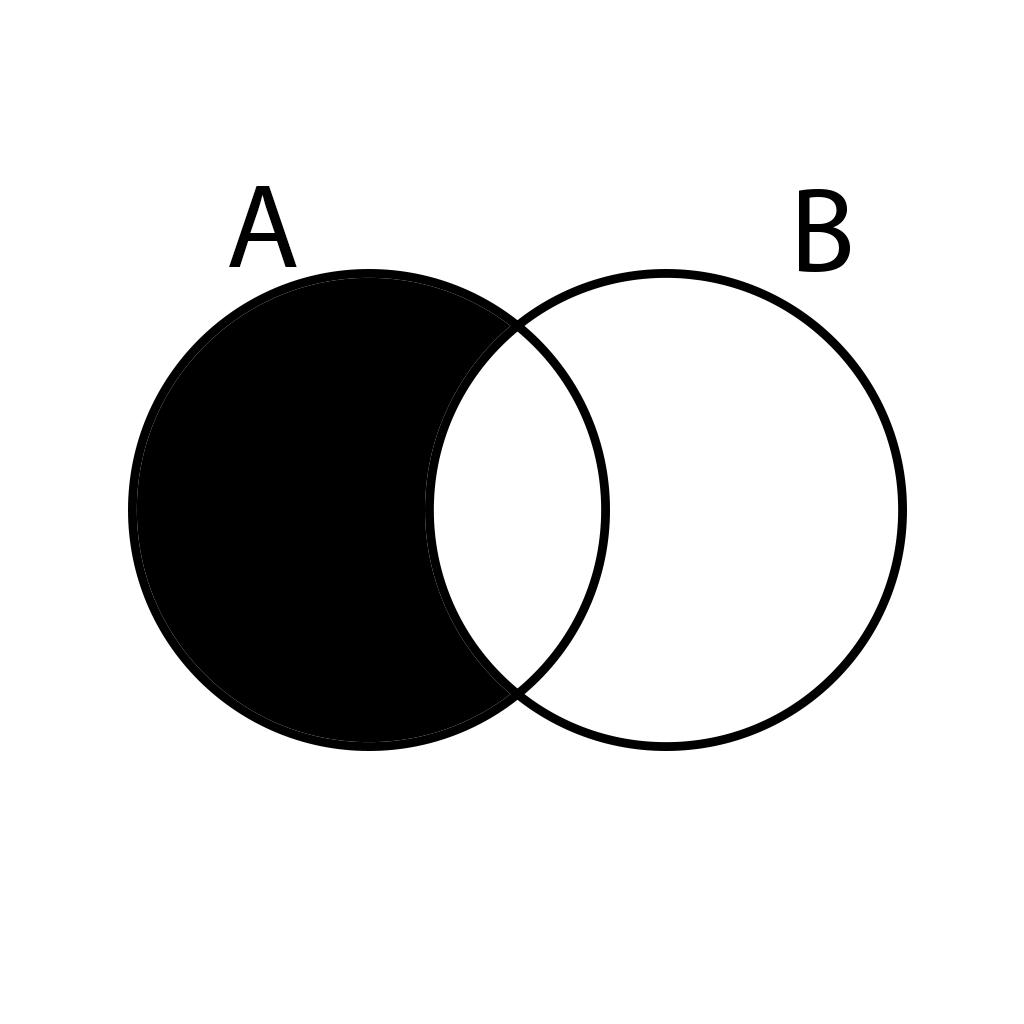
\includegraphics[width=\linewidth]{AVenn}
    \end{minipage}
    &
    \begin{minipage}{.22\textwidth}
      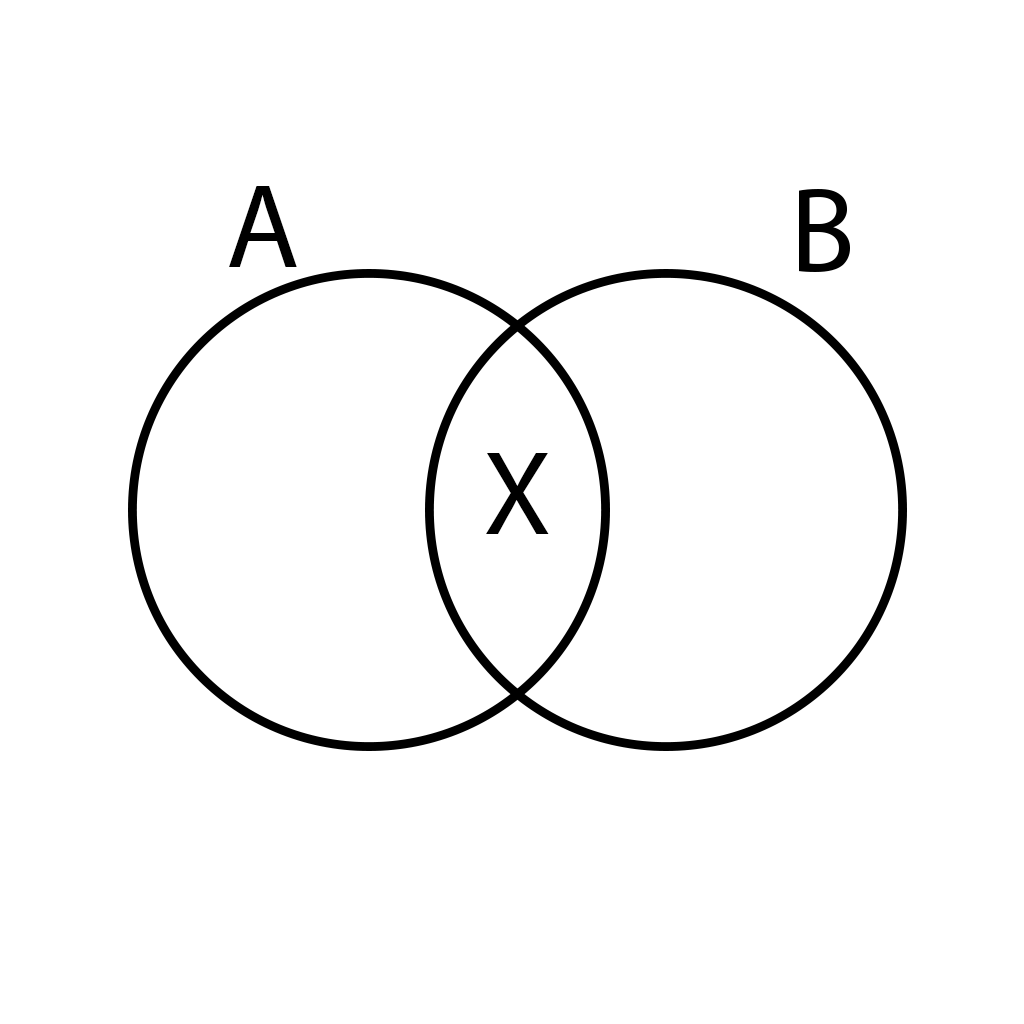
\includegraphics[width=\linewidth]{IVenn}
    \end{minipage}
    & 
    \begin{minipage}{.22\textwidth}
      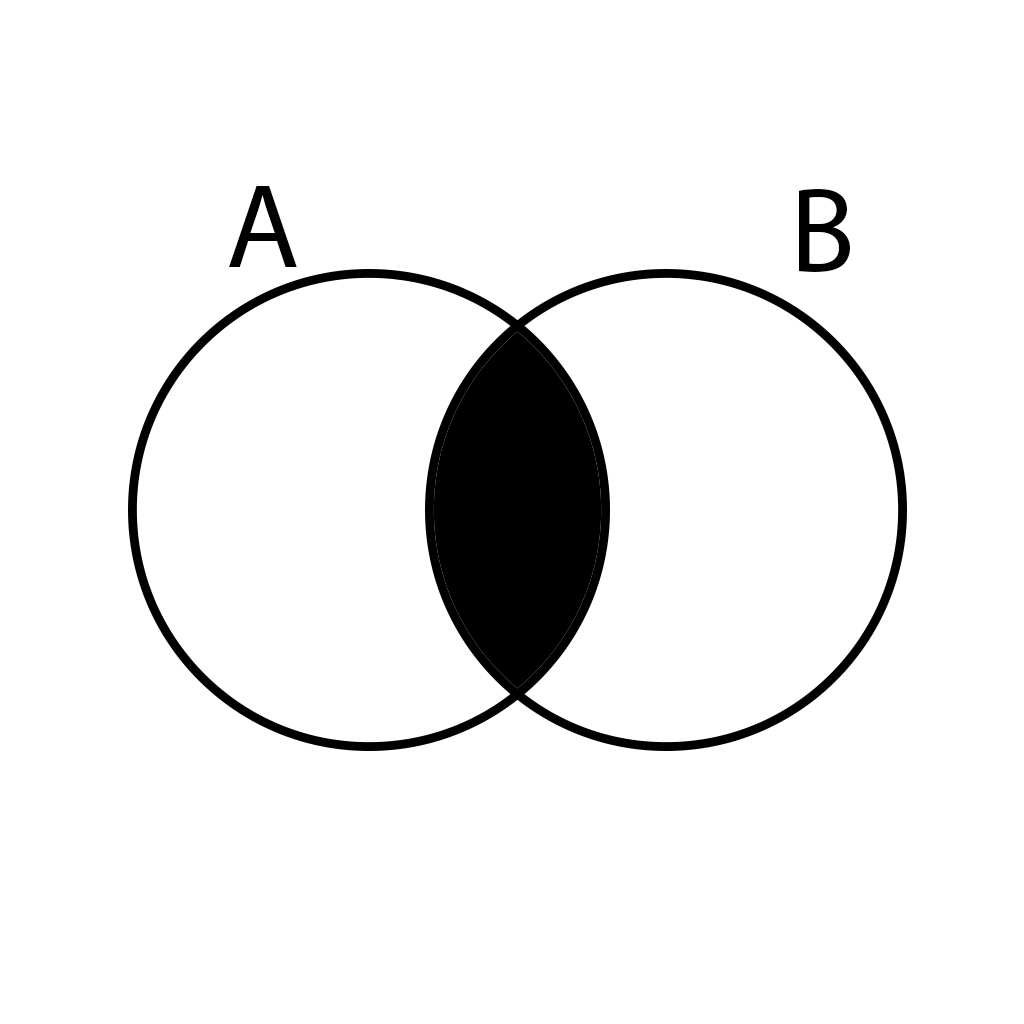
\includegraphics[width=\linewidth]{EVenn}
    \end{minipage}
    &
    \begin{minipage}{.22\textwidth}
      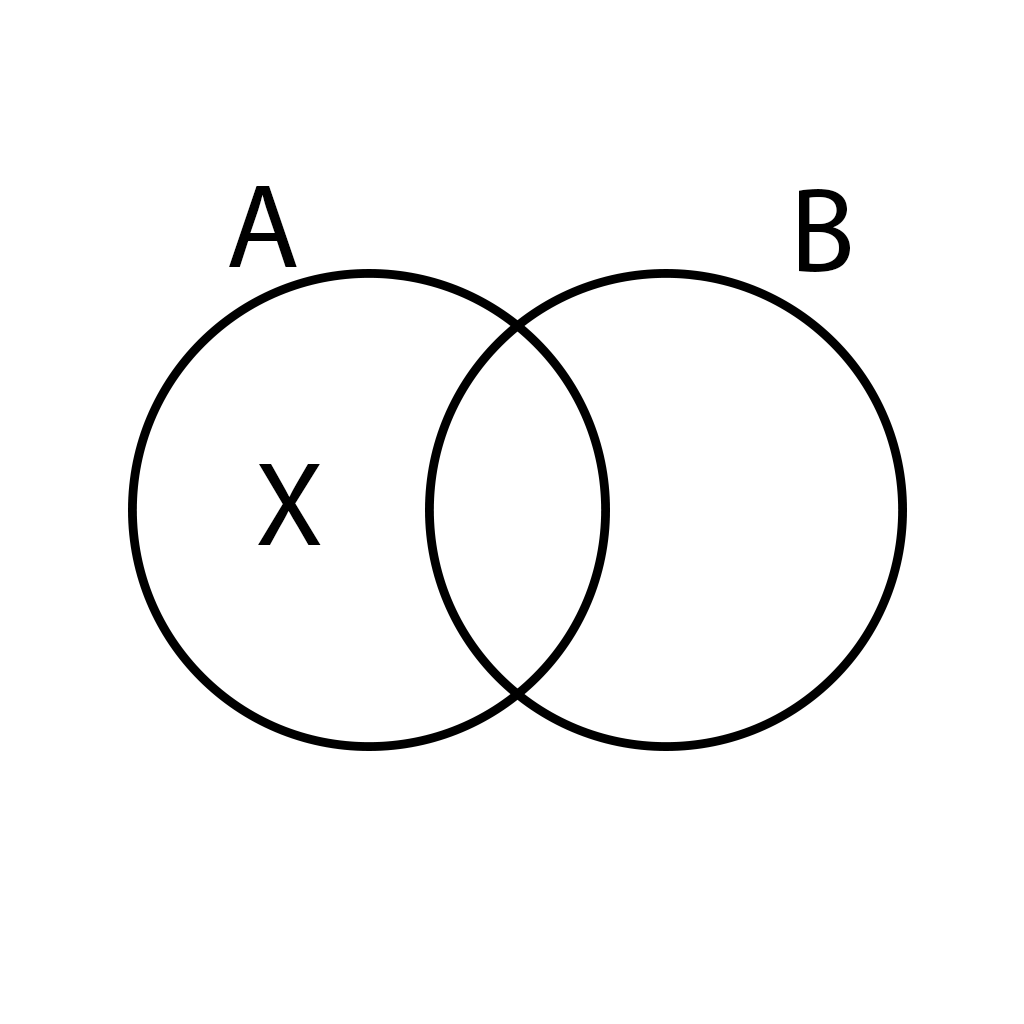
\includegraphics[width=\textwidth]{OVenn}
    \end{minipage}
    \\
  \end{tabular}
  \caption{Premises represented by Venn Diagrams}\label{tbl:vennPremises}
\end{table}

\begin{table}[htb]
  \centering
\begin{tabular}{>{\raggedright\arraybackslash}m{40mm} m{40mm} m{40mm}}
    \multicolumn{1}{>{\centering\arraybackslash}m{40mm}}{\textbf{All Men Are Mortal}} 
    & \multicolumn{1}{>{\centering\arraybackslash}m{40mm}}{\textbf{All Greeks Are Men}} 
    & \multicolumn{1}{>{\centering\arraybackslash}m{40mm}}{\textbf{All Greeks Are Mortal}}\\

    \begin{minipage}{.29\textwidth}
    \begin{center}
      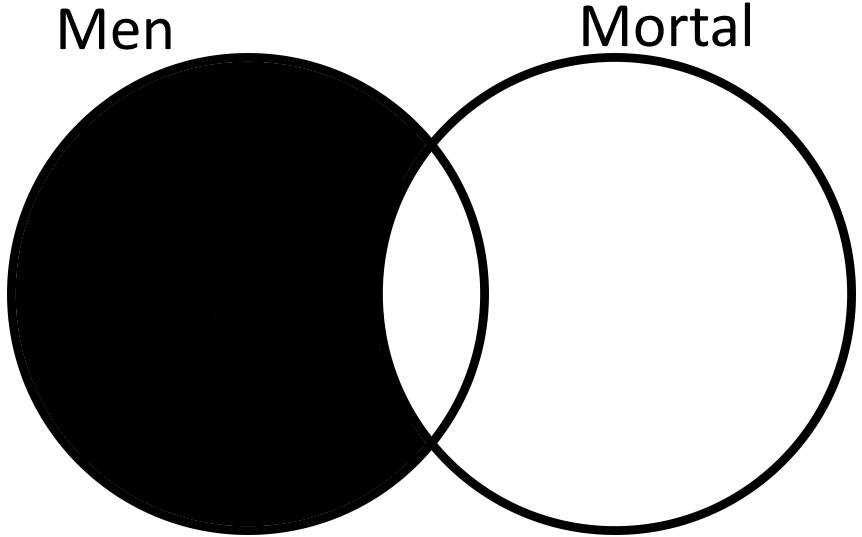
\includegraphics[scale=0.25]{VennAllMenAreMortal}
    \end{center}
      
    \end{minipage}
    &
    \begin{minipage}{.29\textwidth}
    \begin{center}
      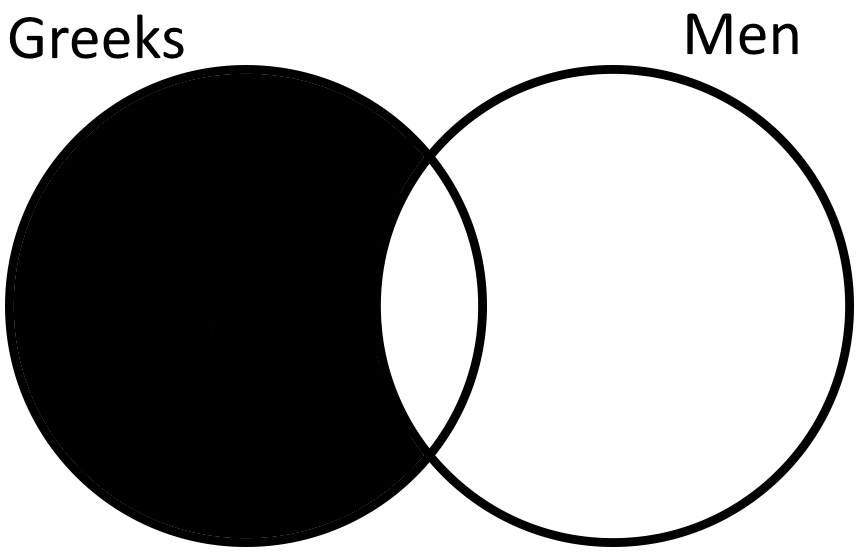
\includegraphics[scale=0.25]{VennAllGreeksAreMen}
    \end{center}
      
    \end{minipage}
    & 
    \begin{minipage}{.29\textwidth}
    \begin{center}
      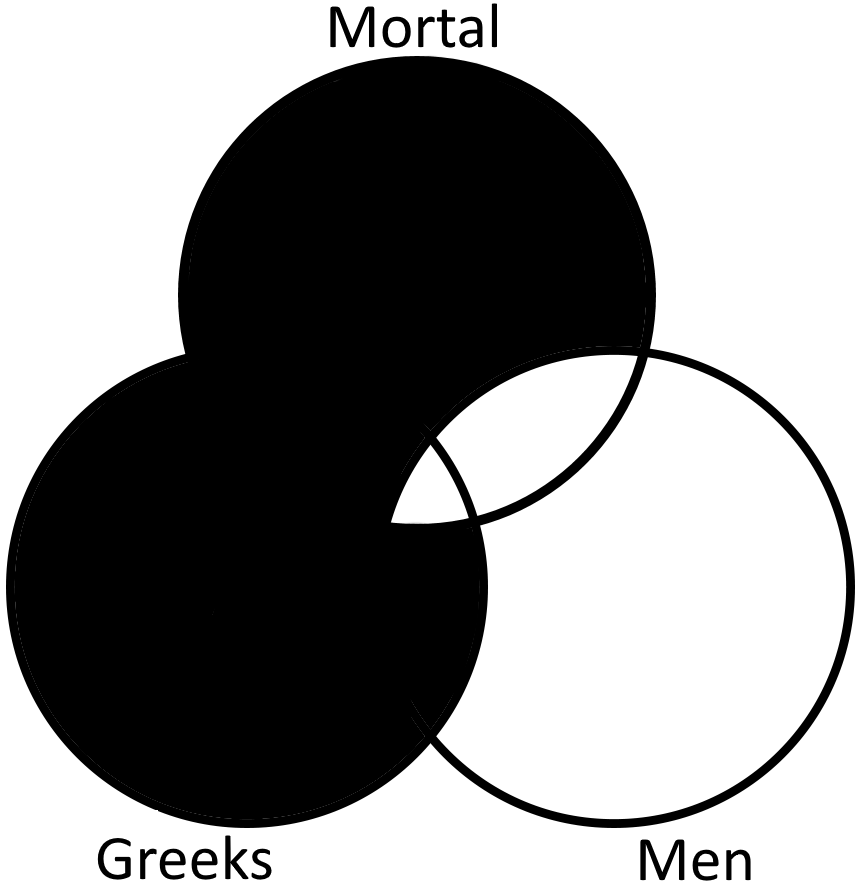
\includegraphics[scale=0.16]{VennAllGreeksAreMortal}
    \end{center}
  
    \end{minipage}
    \\
  \end{tabular}
  \caption{AAA-1 Syllogism}\label{tbl:vennAAA-1}
\end{table}
\FloatBarrier

\begin{table}[htb]
  \centering
\begin{tabular}{>{\raggedright\arraybackslash}m{40mm} m{40mm} m{40mm}}
    \multicolumn{1}{>{\centering\arraybackslash}m{40mm}}{\textbf{No lizards are mammals}} 
    & \multicolumn{1}{>{\centering\arraybackslash}m{40mm}}{\textbf{All lizards are reptiles}} 
    & \multicolumn{1}{>{\centering\arraybackslash}m{40mm}}{\textbf{Some reptiles are not mammals}}\\
    \begin{minipage}{.29\textwidth}
    \begin{center}
    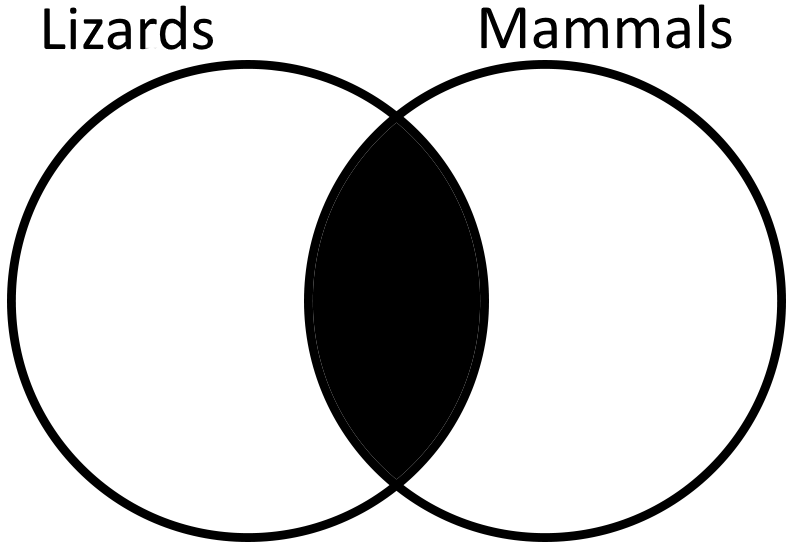
\includegraphics[scale=0.25]{VennNoLizardsAreMammals}
    \end{center}
      
    \end{minipage}
    &
    \begin{minipage}{.29\textwidth}
    \begin{center}
    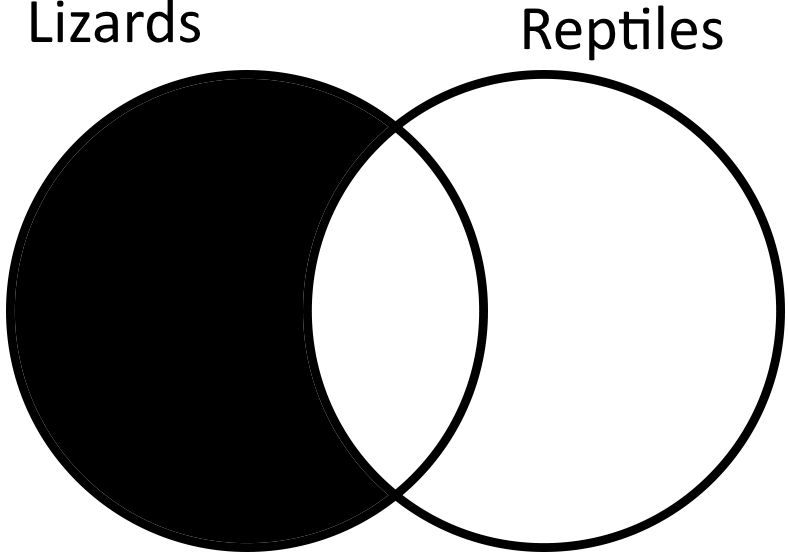
\includegraphics[scale=0.25]{VennAllLizardsAreReptiles}
    \end{center}
      
    \end{minipage}
    & 
    \begin{minipage}{.29\textwidth}
    \begin{center}
     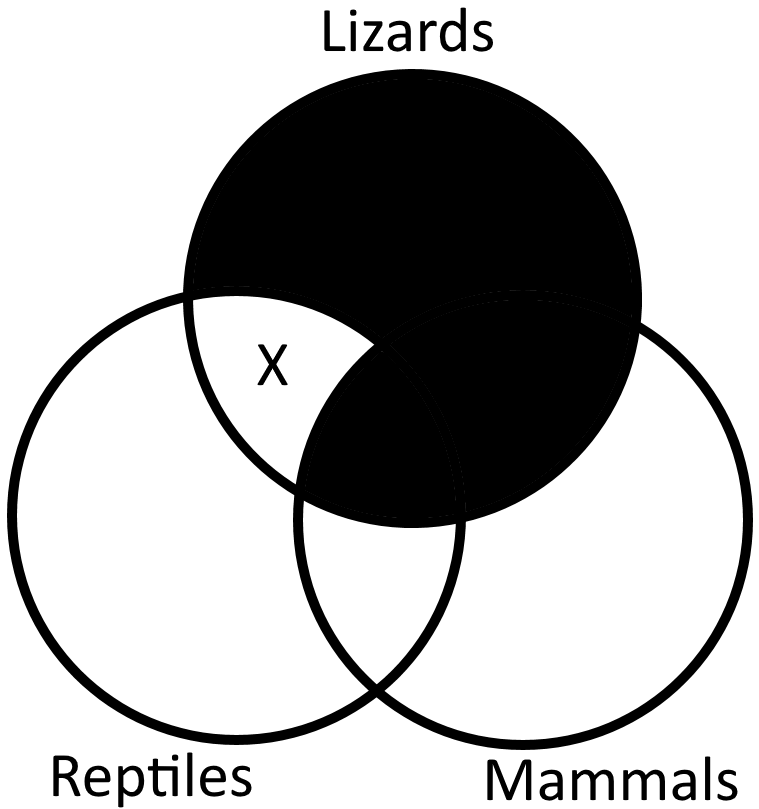
\includegraphics[scale=0.25]{VennSomeReptilesAreNotMammals}
    \end{center}
  
    \end{minipage}
    \\
  \end{tabular}
  \caption{EAO-3 Syllogism}\label{tbl:vennEAO-3}
\end{table}
\FloatBarrier



\subsubsection{Euler Circles}
Euler circles are another popular way in which syllogisms can be represented. 
These are a very natural way of representing sets, with \cite{Erickson1978-ERIROS} putting forward the theory that when people are thinking about syllogisms that they are in fact being mentally thought of as Euler circles. As table \ref{tbl:eulerPremises} shows, when used to represent the individual premises Euler circles can be very intuitive.

%Cirles are 8.5cm I think
\begin{table}[h!]
  \centering
  \begin{tabular}{  c  c  c  c }
    A & I & E & O\\
    \begin{minipage}{.22\textwidth}
      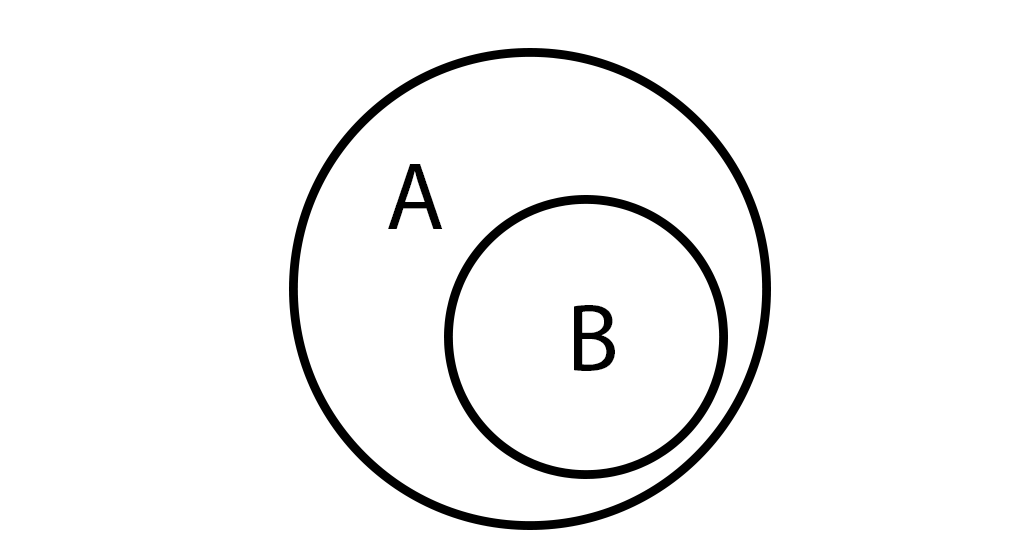
\includegraphics[width=\linewidth]{AEuler}
    \end{minipage}
    &
    \begin{minipage}{.22\textwidth}
      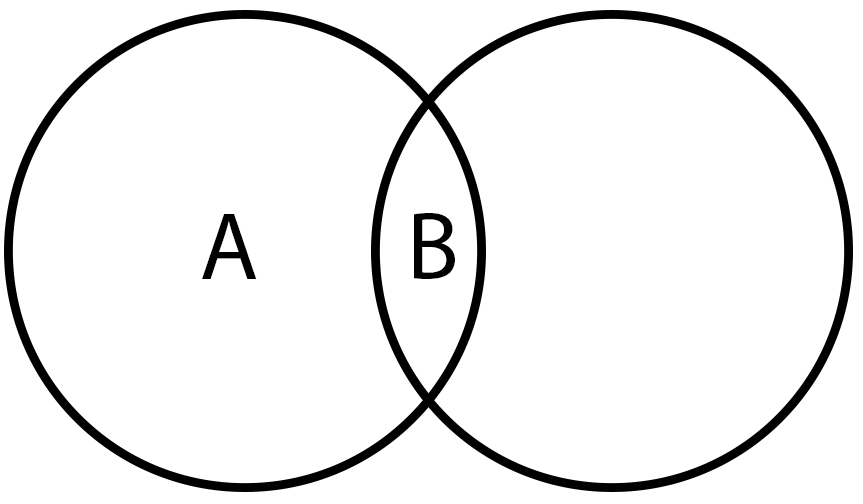
\includegraphics[width=\linewidth]{IEuler}
    \end{minipage}
    & 
    \begin{minipage}{.22\textwidth}
      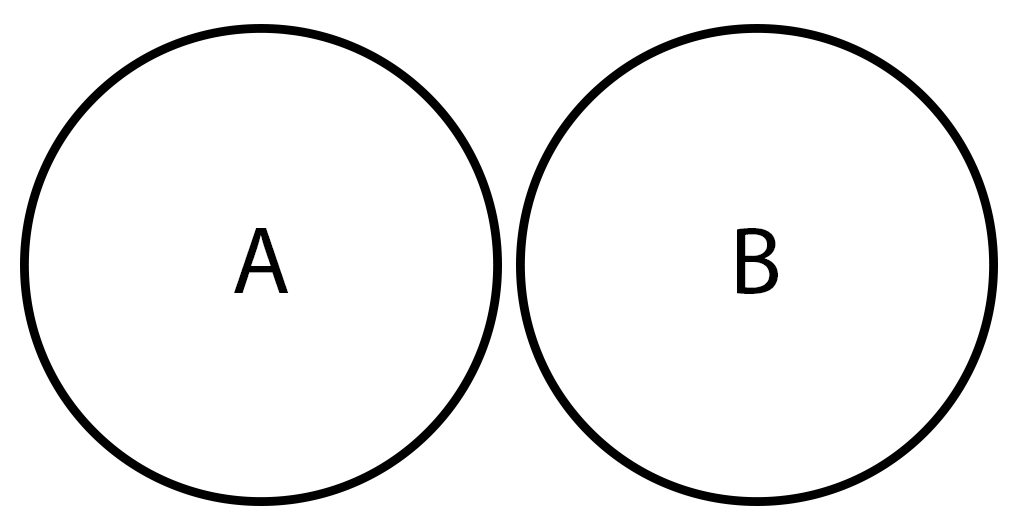
\includegraphics[width=\linewidth]{EEuler}
    \end{minipage}
    &
    \begin{minipage}{.22\textwidth}
      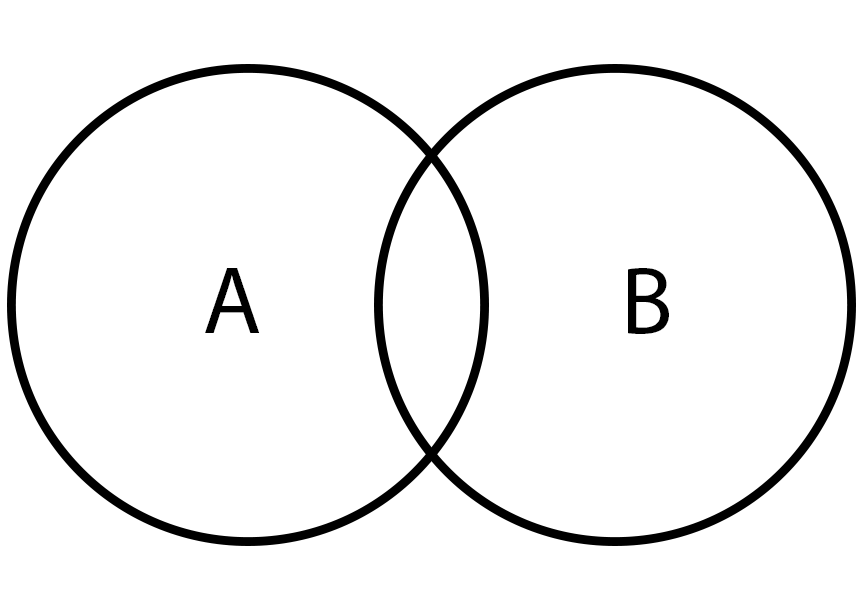
\includegraphics[width=\textwidth]{OEuler}
    \end{minipage}
    \\
  \end{tabular}
  \caption{Premises represented by Euler Circles}\label{tbl:eulerPremises}
\end{table}



\begin{table}[htb]
  \centering
  \begin{tabular}{ c  c  c }
    All Men Are Mortal & All Greeks Are Men & All Greeks Are Mortal\\
    \begin{minipage}{.29\textwidth}
        \begin{center}
             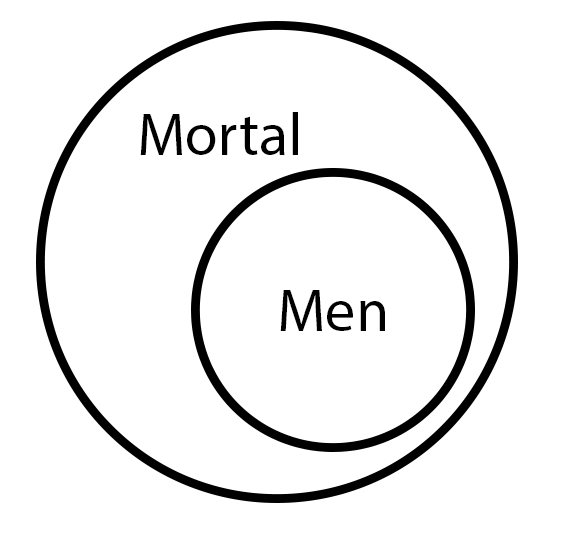
\includegraphics[scale=0.25]{EulerAllMenAreMortal}
         \end{center}
    \end{minipage}
    &
    \begin{minipage}{.29\textwidth}
         \begin{center}
              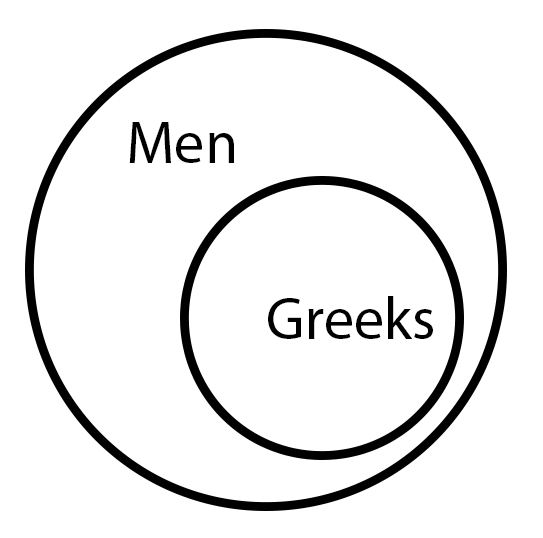
\includegraphics[scale=0.25]{EulerAllGreeksAreMen}
         \end{center}
    \end{minipage}
    & 
    \begin{minipage}{.29\textwidth}
         \begin{center}
         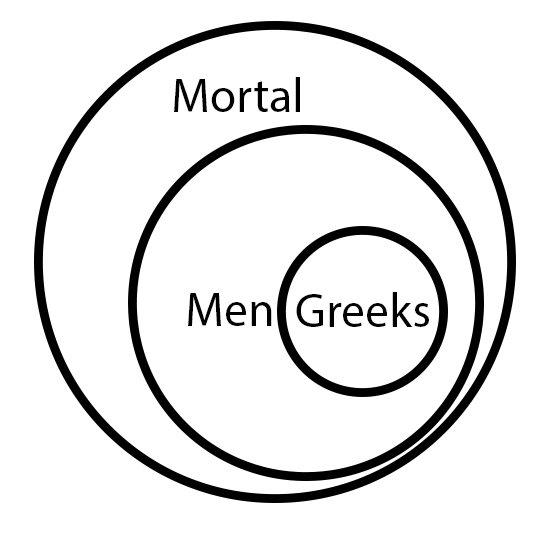
\includegraphics[scale=0.25]{EulerAllGreeksAreMortal}
    \end{center}
    \end{minipage}
    \\
  \end{tabular}
  \caption{Premises represented by Euler Circles}\label{tbl:eulerAllMenMortal}
\end{table}
\FloatBarrier
Euler circles also concisely represents simpler syllogisms as table \ref{tbl:eulerAllMenMortal} shows. However, the problem with this representation arises when more complex syllogisms are constructed. When there are multiple ways to represent the conclusion the result needs more than one diagram to depict all of the possibilities as seen in table \ref{tbl:eulerHomework} . It is at this point that the intuitive benefits are quickly outweighed by the added overhead of managing multiple conclusive diagrams.

\begin{table}[h!]
  \centering
  \begin{tabular}{  c  c  c }
    No homework is fun & Some reading is homework & Some reading is not fun\\
    \begin{minipage}{.22\textwidth}
      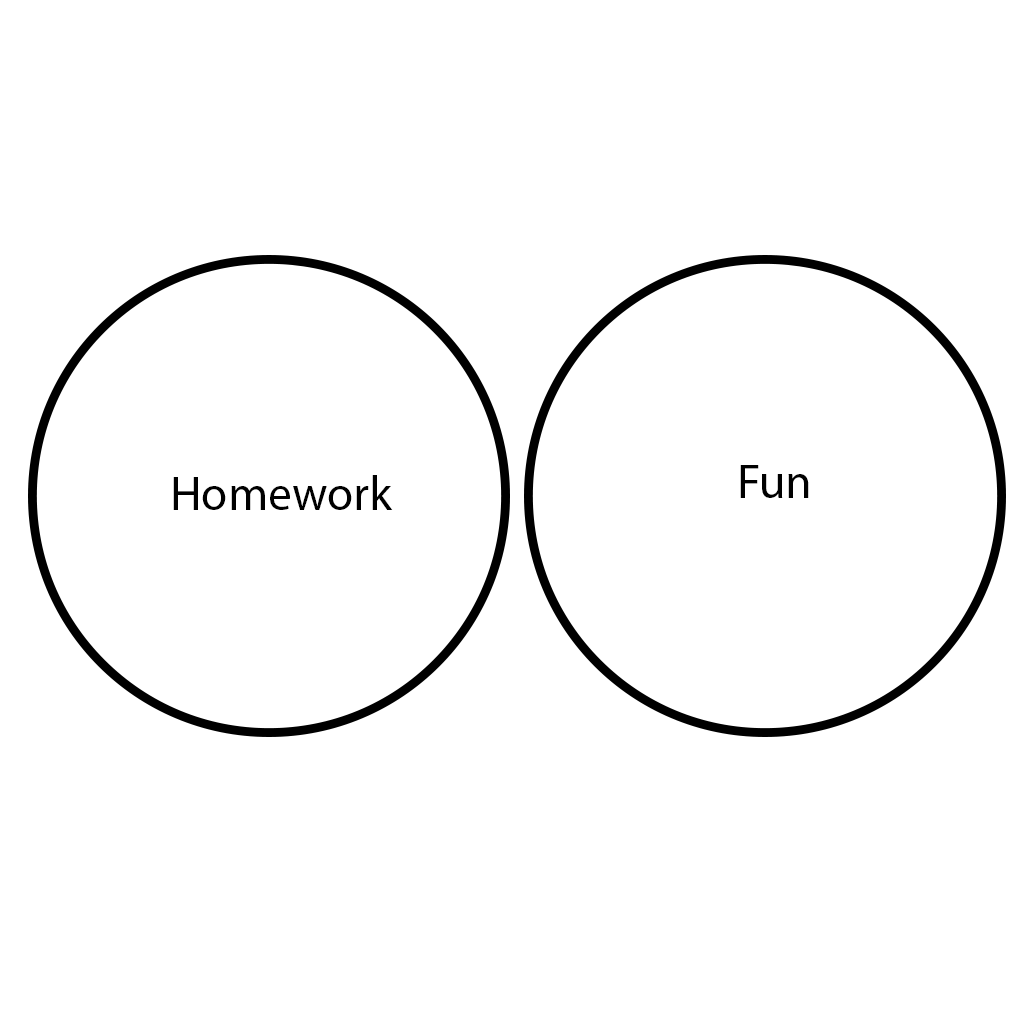
\includegraphics[width=\linewidth]{EulerNoHomeworkFun}
    \end{minipage}
    &
    \begin{minipage}{.22\textwidth}
      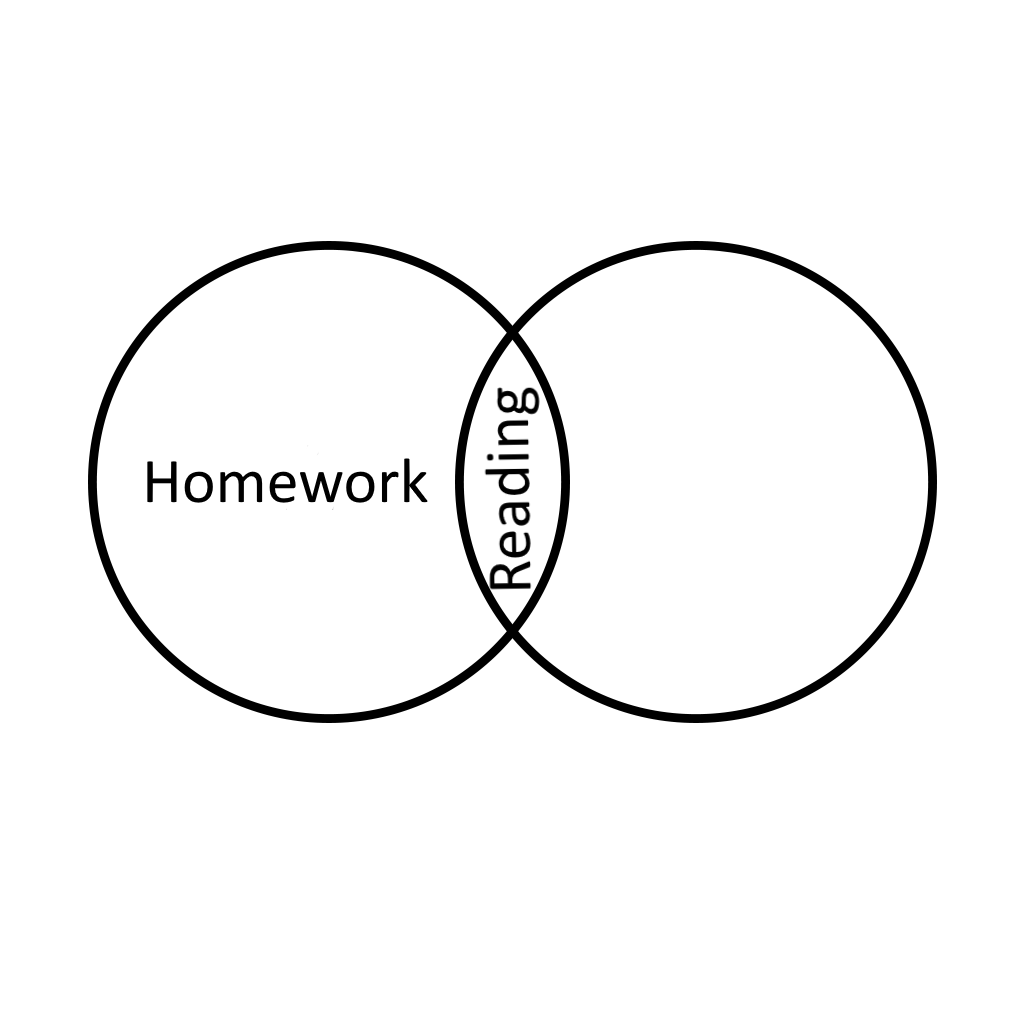
\includegraphics[width=\linewidth]{EulerSomeReadingIsHomework}
    \end{minipage}
    & 
    \begin{minipage}{.22\textwidth}
      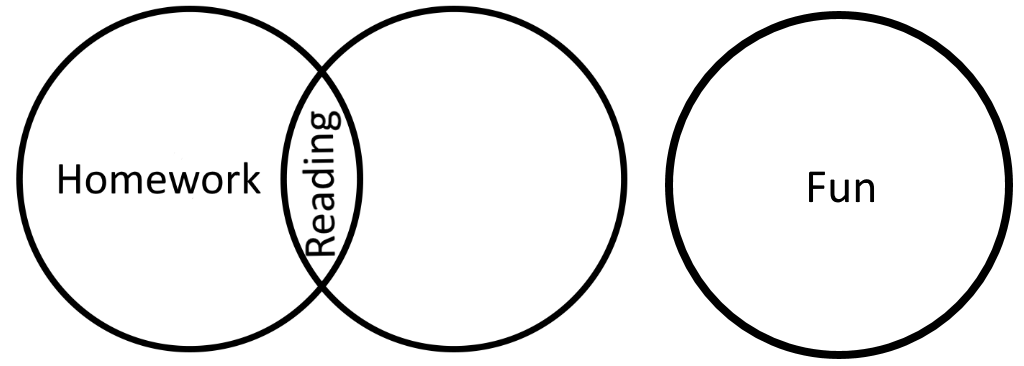
\includegraphics[width=\linewidth]{EulerSomeReadingIsNotFun1}
    \end{minipage}
    \\
    &
     &
    \begin{minipage}{.22\textwidth}
      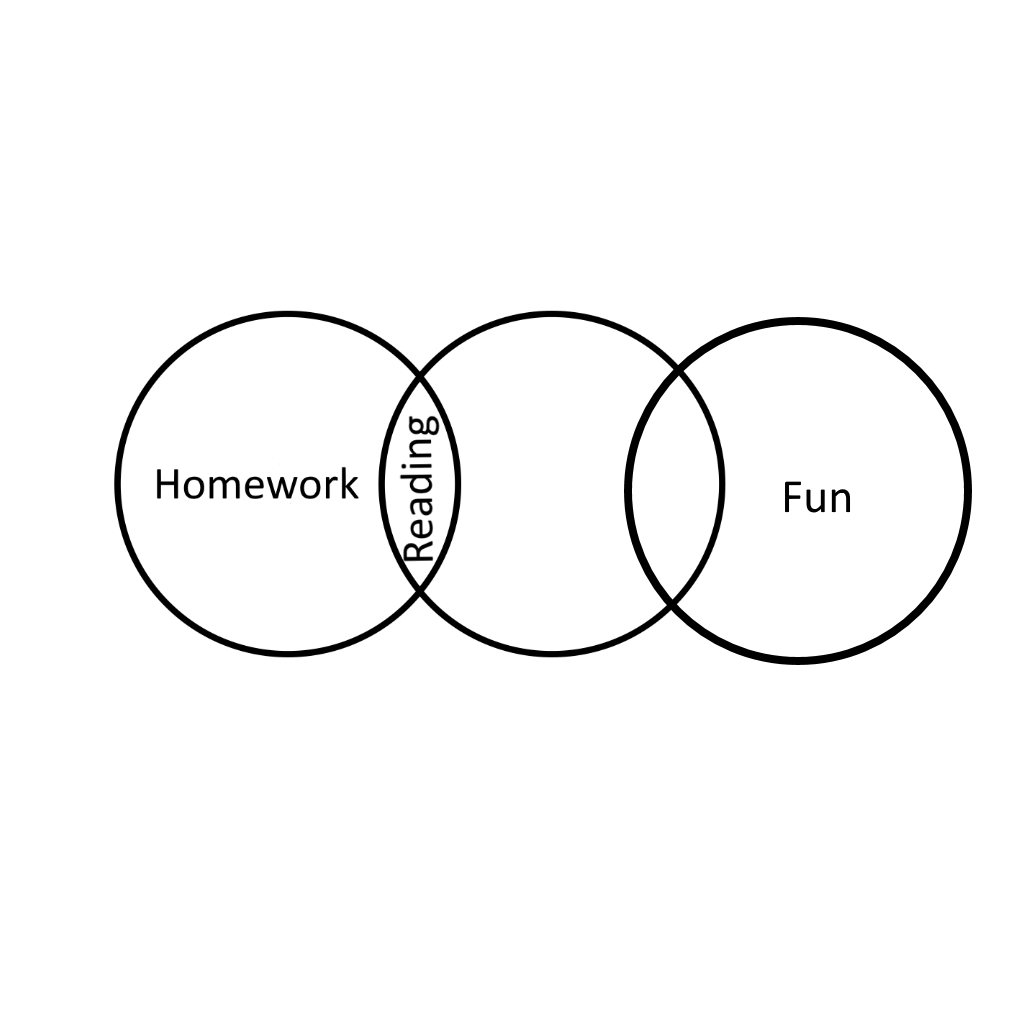
\includegraphics[width=\textwidth]{EulerSomeReadingIsNotFun2}
    \end{minipage}
    \\
    &
     &
    \begin{minipage}{.22\textwidth}
      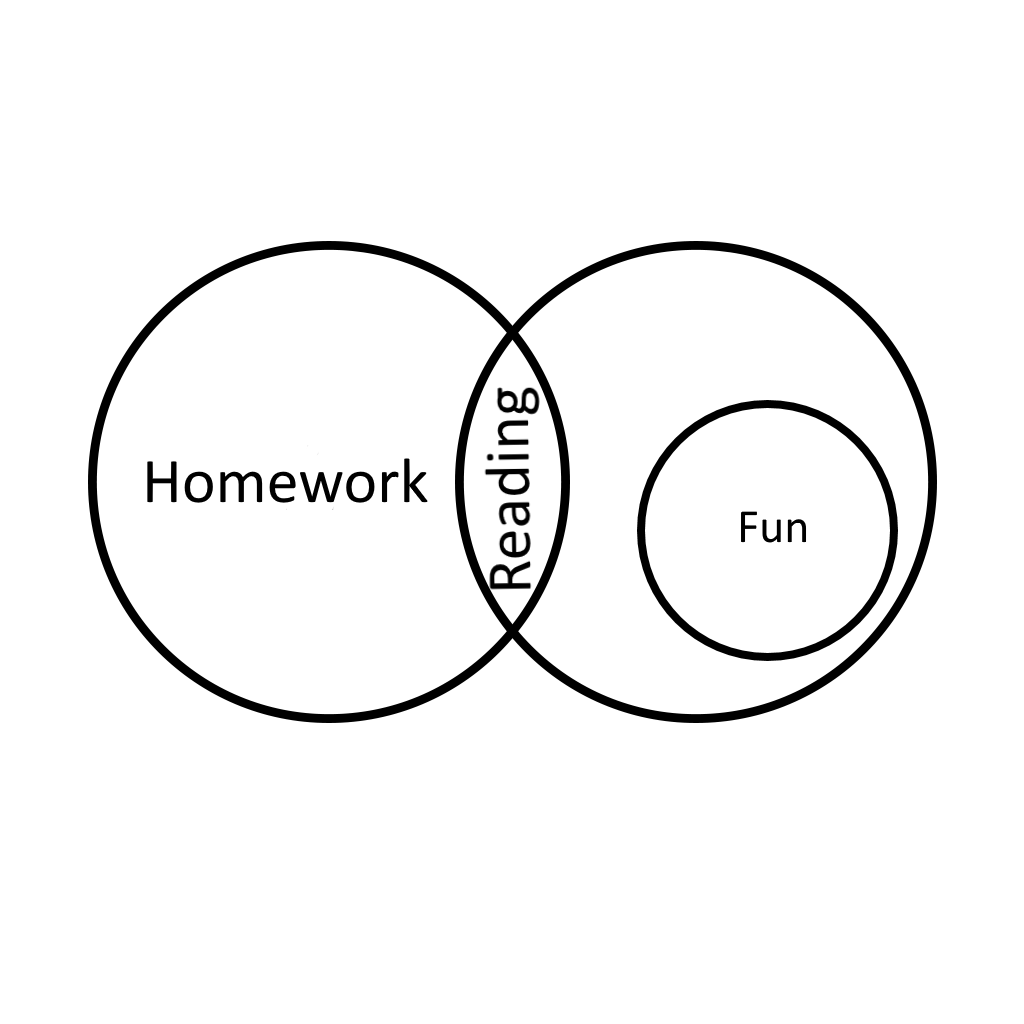
\includegraphics[width=\textwidth]{EulerSomeReadingIsNotFun3}
    \end{minipage}
    \\
  \end{tabular}
  \caption{EIO Syllogism}\label{tbl:eulerHomework}
\end{table}
\FloatBarrier


\subsubsection{Linear Diagrams}
Linear diagrams are an alternative system that was devised by \cite{englebretsen1991}. As the name suggests they are linear instead planar like Venn and Euler diagrams. The reasoning behind this was that Englebretsen said it allowed linear diagrams to represent 4 terms, unlike their planar counterparts. Elements are represented by points which are then connected by lines to show sets.

%Cirles are 8.5cm I think
\begin{table}[h!]
  \centering
  \begin{tabular}{  c  c  c  c }
    A & I & E & O\\
    \begin{minipage}{.22\textwidth}
      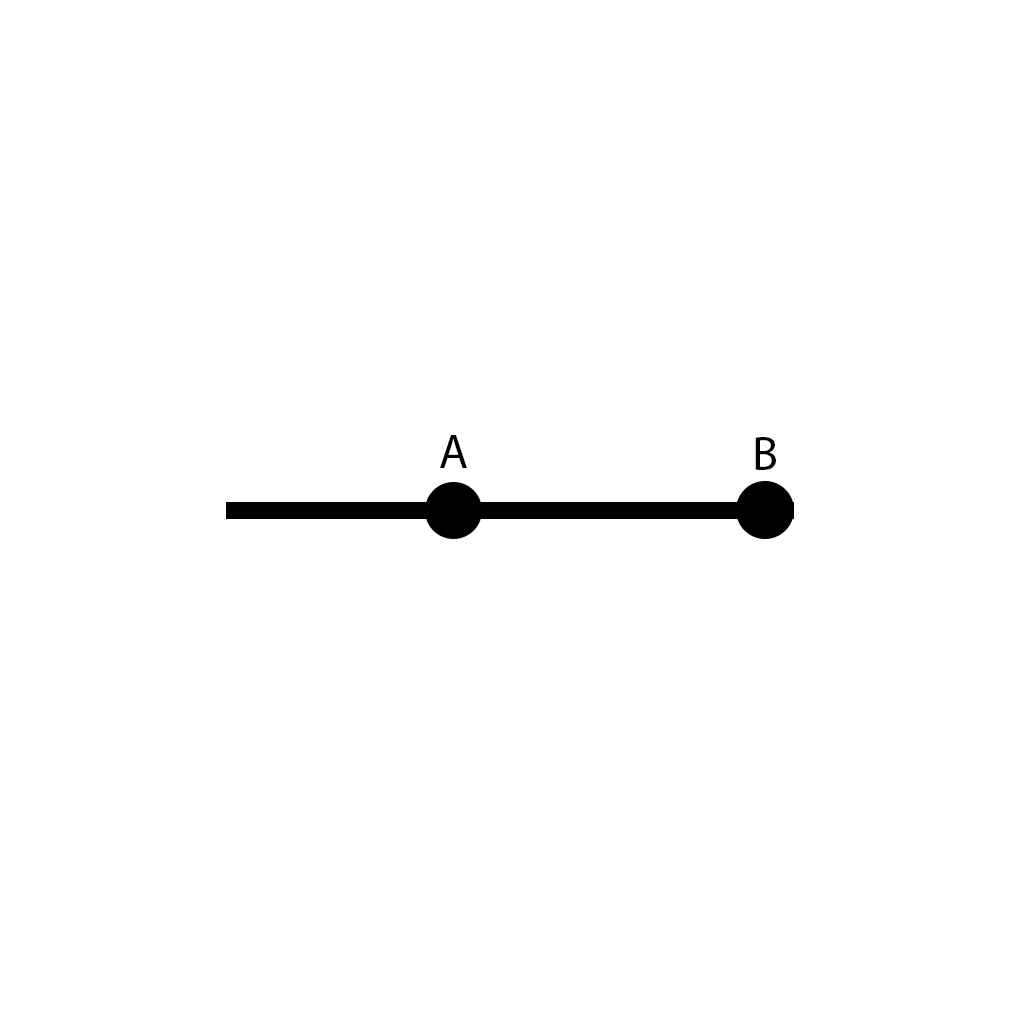
\includegraphics[width=\linewidth]{ALinear}
    \end{minipage}
    &
    \begin{minipage}{.22\textwidth}
      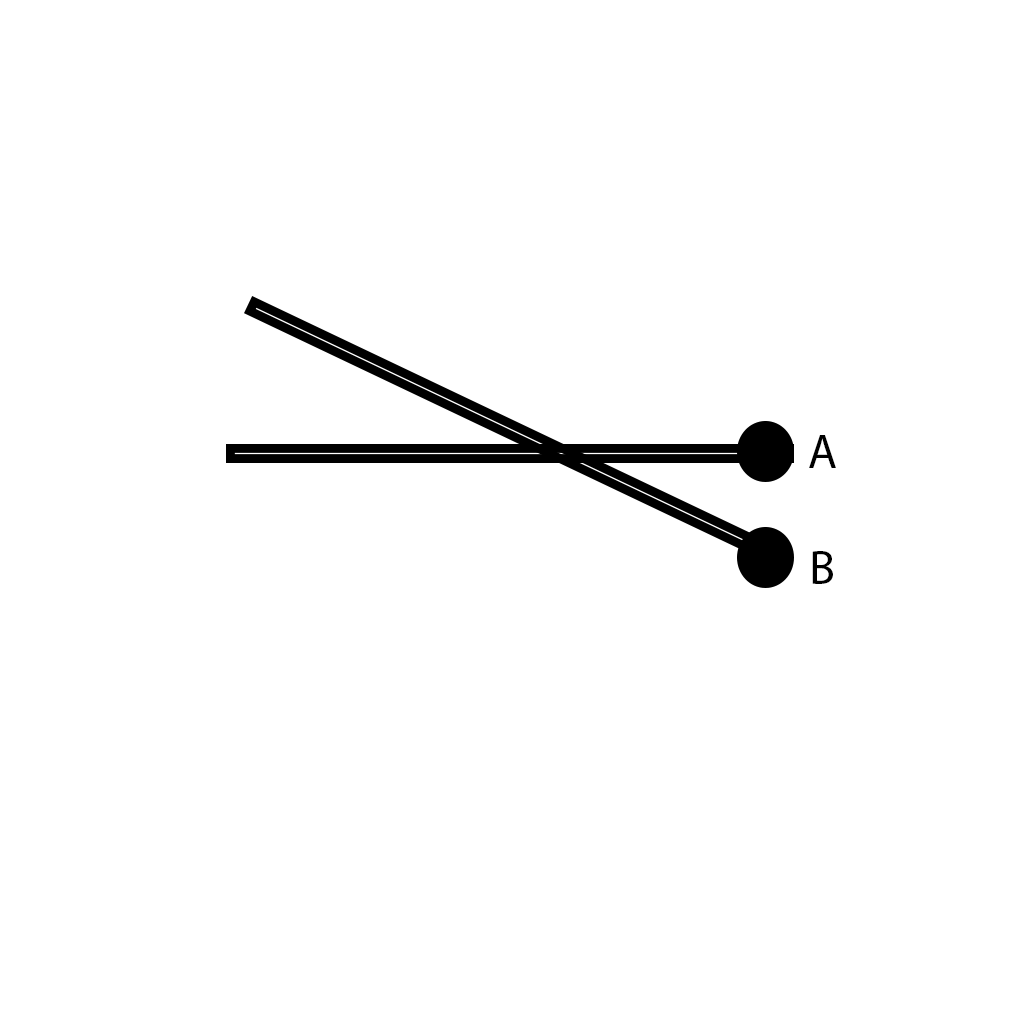
\includegraphics[width=\linewidth]{ILinear}
    \end{minipage}
    & 
    \begin{minipage}{.22\textwidth}
      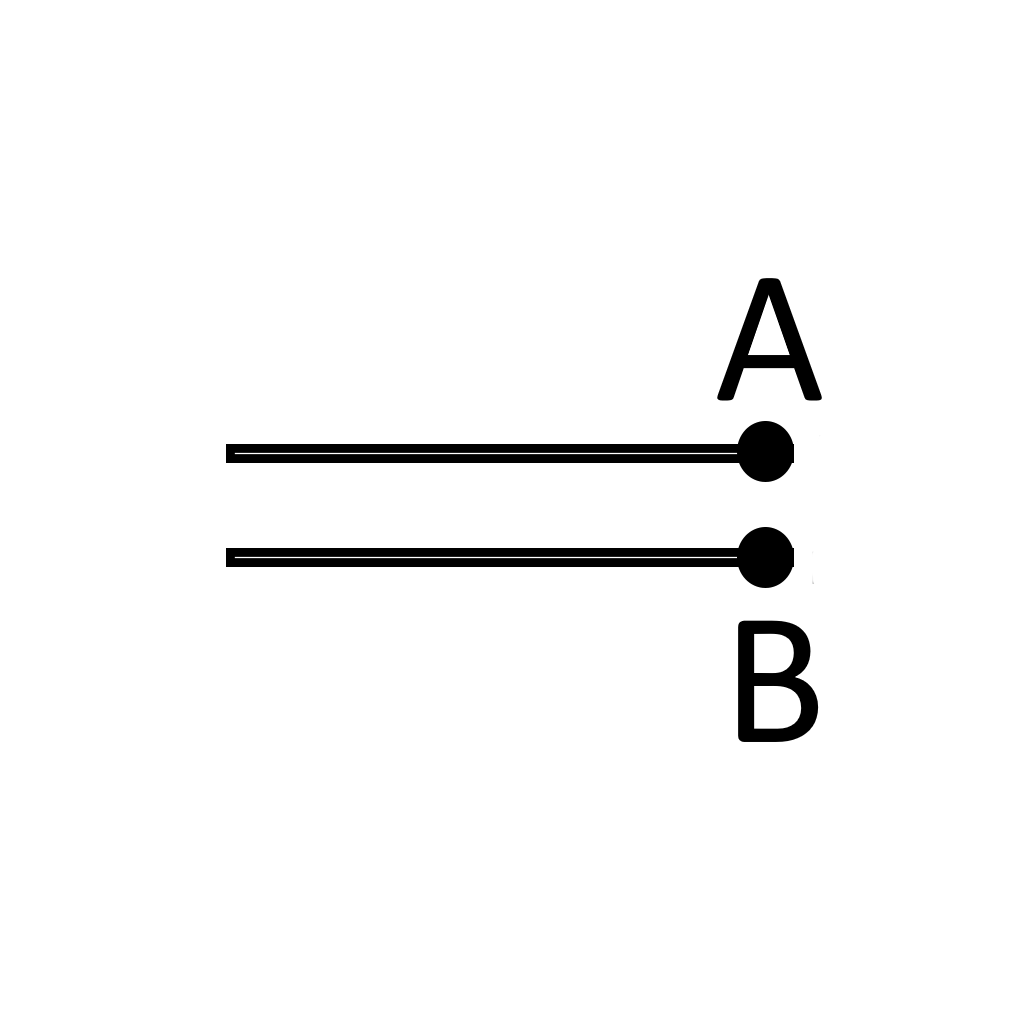
\includegraphics[width=\linewidth]{ELinear}
    \end{minipage}
    &
    \begin{minipage}{.22\textwidth}
      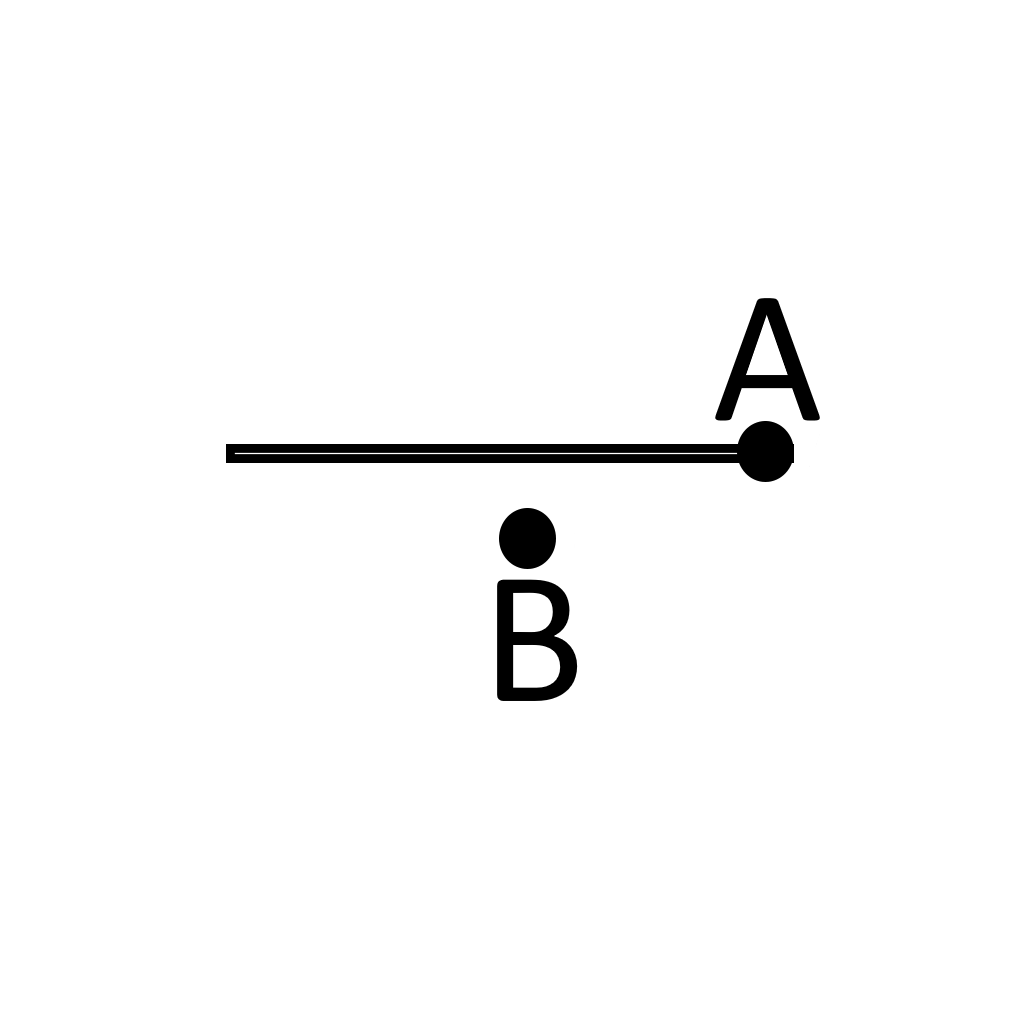
\includegraphics[width=\textwidth]{O1Linear}
    \end{minipage}
    \\
    &
     &
     &
    \begin{minipage}{.22\textwidth}
      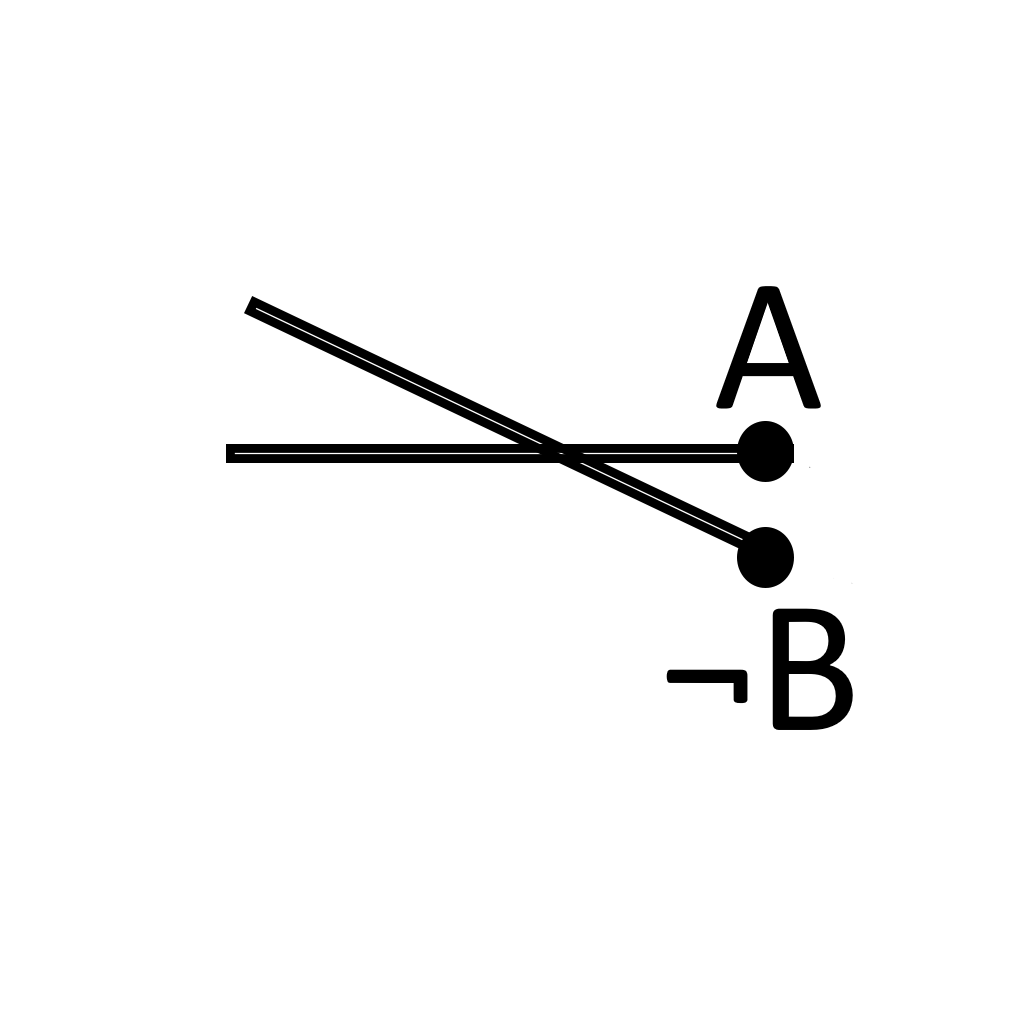
\includegraphics[width=\textwidth]{O2Linear}
    \end{minipage}
    \\
  \end{tabular}
  \caption{Premises represented by Linear Diagrams}\label{tbl:linearPremises}
\end{table}
\FloatBarrier

However, as shown by \cite{lemon1998insufficiency}, linear diagrams do not successfully manage to circumvent the same limitations that planar figures are susceptible to. \cite{lemon1998insufficiency} go as far to say that linear diagrams should only be used for trivial objects and relations and that they are unsuitable for more complex sets.

\subsubsection{Categorical Pattern Diagrams}
As introduced by \cite{cheng2012visualizing}, Categorical Pattern Diagrams offer a relatively new approach with regards to representing syllogisms. The aim behind them is to simplify the process of checking validity, better represent syllogisms with more than 2 premises and generally make the diagrams easier to infer from.

The issue with this form of representation is the notation used is not intuitive. Categorical Pattern Diagrams require the person to learn a whole new notation before they can begin to reason about the syllogism that it is representing.

\begin{table}[h!]
  \centering
  \begin{tabular}{  c  c  c  c }
    A & I & E & O\\
    \begin{minipage}{.22\textwidth}
      
\includegraphics[width=\linewidth, scale=0.5]{CPDA}
    \end{minipage}
    &
    \begin{minipage}{.22\textwidth}
      
\includegraphics[width=\linewidth, scale=0.5]{CPDI}
    \end{minipage}
    & 
    \begin{minipage}{.22\textwidth}
      
\includegraphics[width=\linewidth, scale=0.5]{CPDE}
    \end{minipage}
    &
    \begin{minipage}{.22\textwidth}
      
\includegraphics[width=\textwidth]{CPDO}
    \end{minipage}
    \\
  \end{tabular}
  \caption{Premises represented by Categorical Pattern Diagrams}\label{tbl:cpdPremises}
\end{table}
\FloatBarrier

\subsection{Additional Logic Systems}
So far the only formal logic system looked at has been syllogisms, but many more exist. There are number of systems that would be ideal to include in the syllogism game to allow the player to gain a broader understanding of formal logic.

\subsubsection{Polysyllogisms}
Polysyllogisms, unlike standard syllogisms, can contain more than 3 propositions. This poses a problem for many graphical representations, with traditional circular Venn diagrams being limited to 3 sets. As figure \ref{fig:4SetVenn} and \ref{fig:4SetVenn} show it is possible to represent more than 3 sets using different shapes but as the diagrams become exponentially more complex as sets are added it is quickly becomes impractical to use them.

As reasoned by \cite{cheng2014graphical}, linear and Euler diagrams also struggle with this problem. As both use spatial-overlap it means the diagrams can only represent a series of universal affirmative propositions as further propositions are nested in. As can be seen in table \ref{tbl:linearPremises} and \ref{tbl:eulerHomework} there are already multiple ways to represent syllogisms with 3 terms so it is easy to see how it would quickly become unmanageable as the number of propositions increases.

\begin{figure}[!h]
  \centering
  \begin{minipage}[b]{0.4\textwidth}
    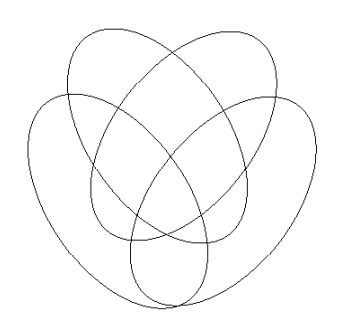
\includegraphics[width=\textwidth]{4SetVennDiagram}
    \caption{4 Set Venn Diagram}
    \label{fig:4SetVenn}
  \end{minipage}
  \hfill
  \begin{minipage}[b]{0.4\textwidth}
    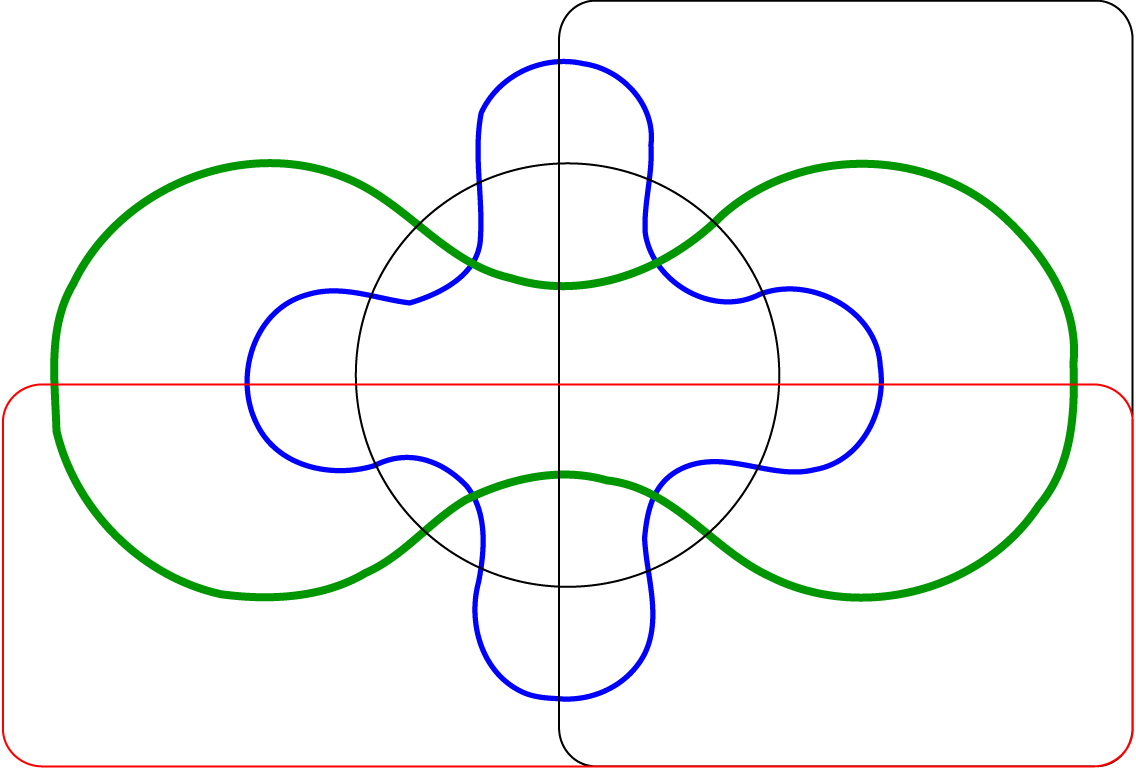
\includegraphics[width=\textwidth]{5SetVennDiagram}
    \caption{5 Set Venn Diagram}
    \label{fig:5SetVenn}
  \end{minipage}
\end{figure}
\FloatBarrier

\subsubsection{Modal Logic}
Modal logic is an extension of classical proposition logic that uses the modal operators \textit{it is possible that} and \textit{it is necessary that} to describe a way in which the rest of the proposition can be true  \citep{zalta1988basic}. Modal logic allows statements to be expressed that would otherwise not be possible in (propositional) classic logic as it is not possible to convey the prospect of events happening. The following are examples of modal propositions:

\bigbreak
\begin{tightcenter}
It is possible that it will snow tomorrow\\
It is necessary that it is either snowing here now or it is not snowing here now.\\
\end{tightcenter}
\bigbreak

The necessity operator is denoted by $\square$, whilst the possibility operator is represented by $\lozenge$.

\subsubsection{Temporal Logic}
Temporal logic is a formal system for specifying and reasoning about propositions with regards to time. It is often used in the formal verification of software systems to interpret concurrent events \citep{lamport1983good}. Temporal logic can be split into two subsections, linear and branching. Linear temporal logic represents time as a set of paths with each part being a sequence of moments. From any given moment there is only one possible future moment, a unique successor. Branching linear logic represents time as a tree with the root as the present and the branches being the future.


\begin{figure}[!h]
  \centering
  \begin{minipage}[b]{0.4\textwidth}
    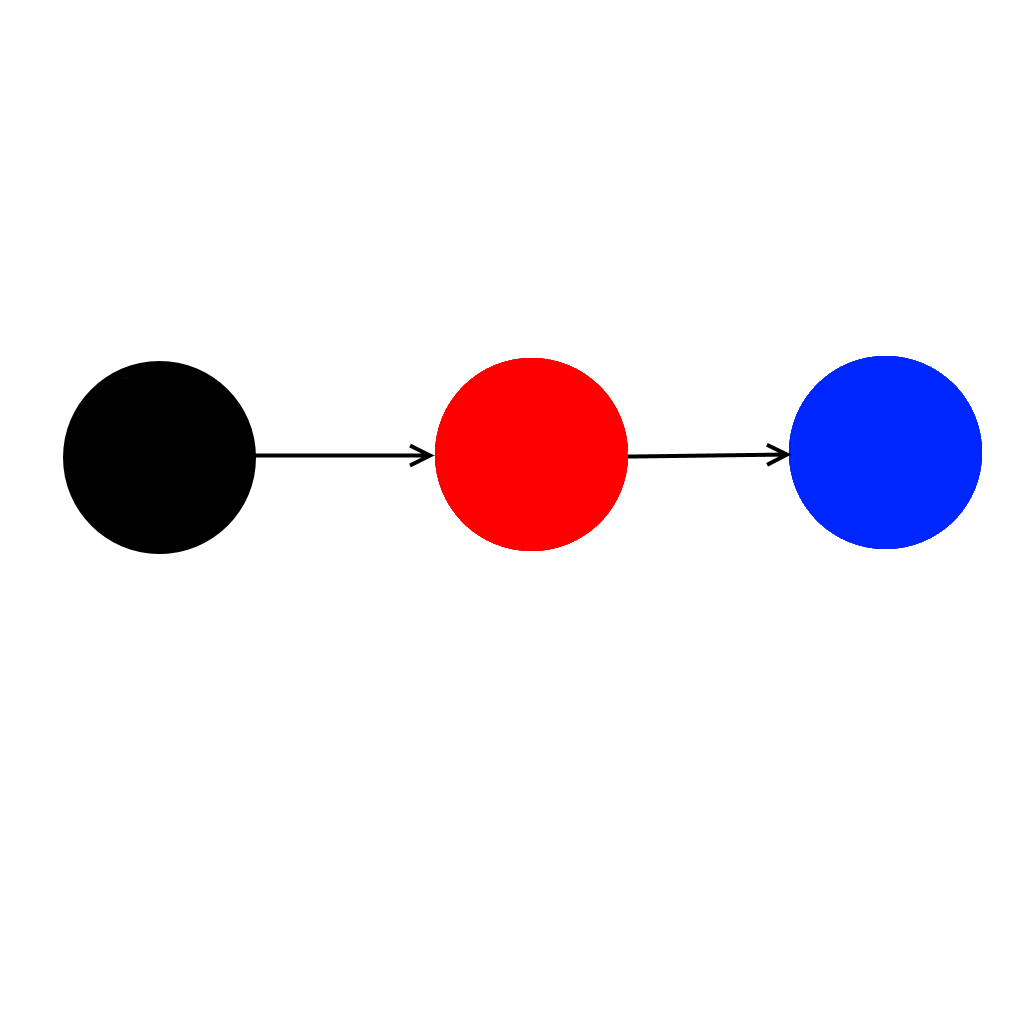
\includegraphics[width=\textwidth]{LinearTemporalLogic}
    \caption{Linear Temporal Logic}
  \end{minipage}
  \hfill
  \begin{minipage}[b]{0.4\textwidth}
    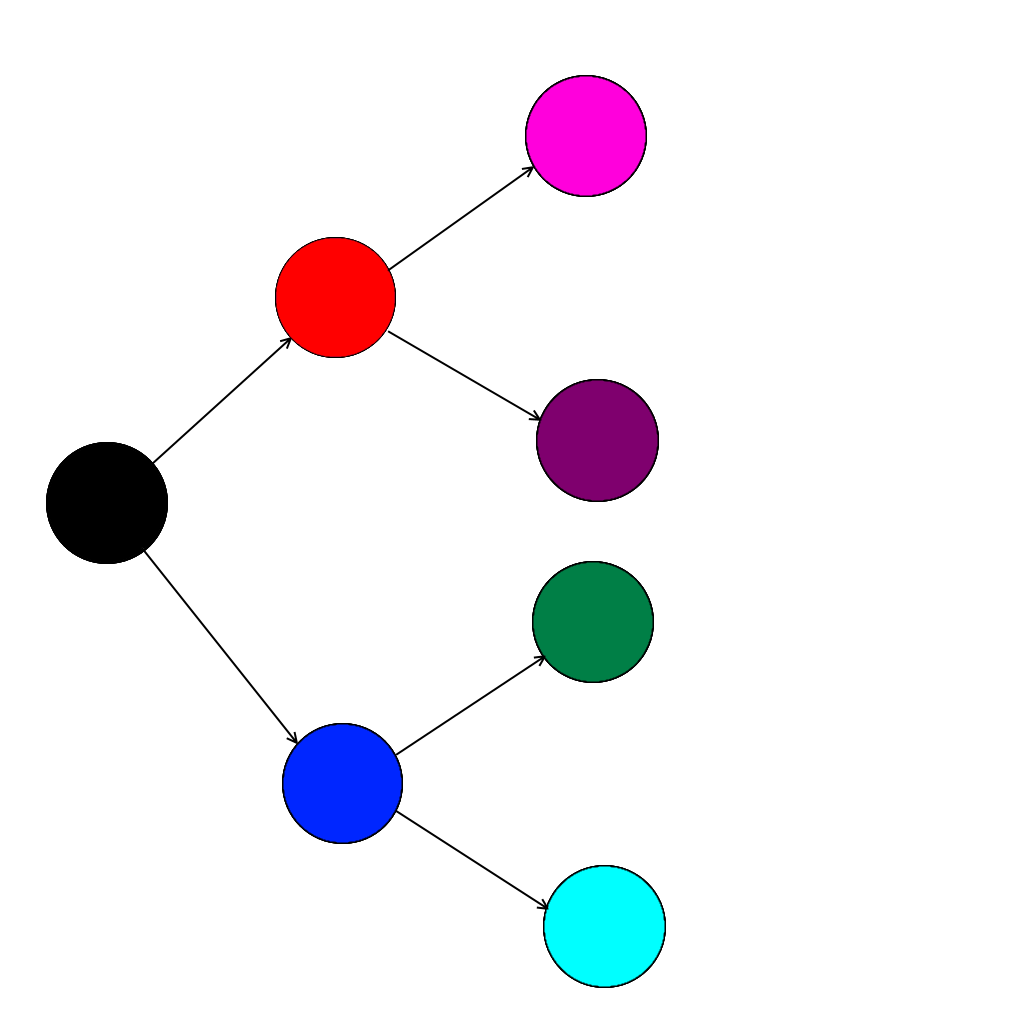
\includegraphics[width=\textwidth]{BranchingTemporalLogic}
    \caption{Branching Temporal Logic}
  \end{minipage}
\end{figure}
\FloatBarrier

\subsubsection{Set Theory}
Set theory is the mathematical theory of well-defined collections known as sets. These sets are made up of objects called elements. Given a set $S$ and an element $x$ it is said $x \in S$ if $x$ is an element of $S$ and conversely $x \notin S$ if $x$ is not an element of $S$ \citep{sep-set-theory}.

Diagrammatically they appear very similar to syllogisms as both utilise Venn diagrams so it would naturally follow on well to expand syllogisms to encompass set theory. This is especially true when it is considered how syllogisms can be represented using set theory notation as in table \ref{tbl:setTheoryNotationTable}.
 
\begin{table}[h!]
\begin{center}
  \begin{tabular}{ c | c | c }
    Syllogism & Set Notation & Sentential Representation \\ \hline
    AaB & $B \subseteq A$ & All B is A \\
    AiB & $B \cap A \neq \emptyset$ & Some B is A \\
    AeB & $B \cap A = \emptyset$ & No B is A \\
    AoB & $B \cap A \nsubseteq B$ & Some B is not A \\
  \end{tabular}
   \caption{Set Theory Notation for Syllogisms}
  \label{tbl:setTheoryNotationTable}
\end{center}
\end{table}


\section{Serious Games}
\subsection{Introduction}
Serious Games are a movement within the game industry comprised of software developers and researchers who are using games to educate. Whilst there is some debate around what exactly construes a serious game, \cite{michael2005serious} define one as any game where entertainment is not the primary purpose, but where instead the focus is on education. They aim to tackle a growing problem whereby educational techniques have not adapted to the needs of the current generation. As \cite{lim2008spirit} discusses, learning in the classroom has been driven by the national curriculum, with a massive focus on standard and grades. This goes against the belief that to attract the attention of students the focus should in fact be on creating an engaging learning environment. In contrast with previous generations, the younger generation of today have grown up in a world consumed in technology. \cite{oblinger2005educating} described them as the \textit{Net Generation}, the generation who always need to be connected, require immediate feedback and crave social interaction. The research of \cite{prensky2001games} explains how this vast amount of technology now experienced in everyday life has led to these newer generations having their minds rewired. These cognitive changes have caused a different set of educational preferences when compared to previous generations, with teaching methods not evolving in order to take this into account.

\subsection{Why They Are Good For Education}
\subsubsection{Accessibility}
One of the benefits of using games to teach is their accessibility in comparison to other methods. In the United Kingdom  access to the internet has doubled over the past 10 years, with 82\% of adults now using the internet on a daily basis \citep{onssurvey}. With such a huge number of people using the internet it means that games hosted on the web have an extremely large potential audience. This broad audience coupled with the widespread appeal of video games allows the crossing of demographic boundaries such as age, gender and educational status \citep{griffiths2002educational}.  Serious Games also have a lower barrier to entry than other educational techniques by allowing a much more "pick up and play" approach to learning with less reliance on prerequisite background knowledge. In the case of syllogisms this would be achieved by using graphical representations to replace the set theory notations. By teaching the concepts first, set theory notation could then be introduced at a more appropriate time in the learning process when the player had a greater understanding of the topic. 

\subsubsection{Motivation}
As discussed by \cite{malone1981toward} games can be intrinsically motivating, such that there are no external factors as to why a person is playing other than for their own enjoyment. This is in contrast to typical classroom learning that is usually more extrinsically motivated through grades, exam results and certificates. As  \cite{csikszentmihalyi1997talented} says, the school attendance would see a sharp drop if extrinsic rewards were removed. Of the two, intrinsic motivation is more resilient than extrinsic motivation and learning that takes place as a result of intrinsic motivation is of higher quality and longer lasting \citep{kawachi2003initiating}.

However, it is important to remember that not all games are by definition intrinsically motivating, but need to be structured correctly to achieve this. Malone included challenge, fantasy and curiosity as the three cornerstones of intrinsically motivating serious games.  
In order to create a challenging game, it should include uncertain goals that are not too easy for the players to complete. Ensuring a game is challenging is crucial as demonstrated by Malone's work surveying children's opinion on 25 different computer games. The results conclusively showed that the most popular games all shared one thing in common; they all contained a defined goal.  Similarly in a study carried out by \cite{abuhamdeh2012importance} on chess players, it was found that the more challenging the game the greater the player's enjoyment. This is important to bear in mind with syllogisms as it is demonstrates the need to add the correct amount of difficulty for the game to be successful.

A fantasy environment in a game is said to "evoke mental images of phyical or social situations not actually present". Malone divides these fantasies into intrinsic and extrinsic, with intrinsic being more interesting and instructional resulting in a  greater cognitive effect on learning. \cite{lepper1988motivational} explains how if learning takes place away from the functionality of the knowledge then this decontextualisation results in the learner becoming demotivated.  This can be tackled by using real world examples demonstrating how the concepts are applied. For syllogisms this can just be as simple as using actual examples that exist as opposed to using letters to represent sets. However, as this is not always feasible, Lepper proposed inserting the content of the topic into a fantasy context.
Curiosity, like challenge, is stimulated from an optimal level of complexity. Curiosity is also broken down into two categories; sensory and cognitive.  Sensory curiosity, as the name suggests, uses lights, sounds and graphics to gain the attention of the participant. Cognitive curiosity is achieved by making the participant doubt their existing knowledge, as people desire to have "good form" in their cognitive structure.   By using this taxonomy when developing a serious game, it is clear that this could be used to engage people who otherwise might not have been interested in learning. 

\subsubsection{Feedback}
Feedback is information regarding a person's understanding of a concept provided with the intention of improving the person's ability. Feedback is a crucial part of the education process and significantly influences the effectiveness of learning.

As stated by \cite{hattie2007power}, "feedback is
one of the most powerful influences on learning and achievement". A further study explored the most effective medium to provide feedback. Computer-assisted, audio and video feedback were found to be most effective forms with the more traditional approach of praise, punishment and providing extrinsic rewards being the worst \citep{hattie2007power}. 

One of the main advantages of using games for education is the speed at which feedback can be delivered to the learner which is especially important to the \textit{Net Generation}. The term \textit{fast feedback} was coined by \cite{lumsden1988characteristics} to demonstrate how this timely feedback removed any uncertainty about progress and allowed any corrective action to be taken during the learning process. However, fast feedback is not a silver bullet and as such the speed at which feedback is delivered should depend on the difficulty of the task. The more complex the task, the greater the benefit of delaying the feedback to allow the information to be processed \cite{clariana2000applying}. 

Feedback during the learning process is known as formative assessments, with summative assessments usually being carried out at the end. As explained by \cite{irons2007enhancing}, formative assessments can be beneficial as they enhance the learning process by creating a positive environment which results in greater motivation for learner. 

Serious Games lend themselves extremely well to delivering formative feedback to players through in-game features such as progress bars, score count and countdown timers. Feedback can also be provided to the player as they make mistakes allowing the player to engage with the game and keep on track to completing their goals. This can also help the player from becoming frustrated and unable to progress.

\subsection{Existing Serious Games}
Serious Games can be split into two main categories, mini-games and complex games. Mini Games tend to be far shorter, often only taking less than an hour to complete. The focus is aimed at a very specific topic within a subject and is usually browser based. Progression tends to be added through multiple levels, all with similar design but with increasing difficulty. This is the far more common type of Serious Game as they are far cheaper to develop.

In contrast, complex games can take potentially hundreds of hours to complete and cover a very broad topic. The game may contain multiple skills, paths to follow and complex goals.  

Serious games do not just apply to education, but are used by a wide variety of different industries. The United States military created America's Army to aid in their recruitment and Microsoft's Flight Simulator is used by pilots in training \citep{111701519980901}.


\subsubsection{MyMaths}
MyMaths is a web based service that is used by schools in over 70 countries, with over 4.5 million users. It is marketed as an online learning platform that provides lessons and homework to school children. It allows them to complete all of this work online and is then automatically marked.
As Figure 2.1 shows, MyMaths makes use of fast feedback to provide the player with the results as soon as they have completed the task. However, MyMaths does not provide an immersive or particularly enjoyable experience for players. \cite{lee2013learning} found that while students said they enjoyed using computers to learn, they did not want to use MyMaths. This could be due to that fact that MyMaths is very one dimensional, merely presenting questions in a quiz like format. This does not engage with the player, incite any emotive feelings or provide any fantasy environment. It would more enjoyable if the technologies available were used to make it more interactive.
\begin{figure}[!tbp]
  \centering
  \begin{minipage}[b]{1\textwidth}
    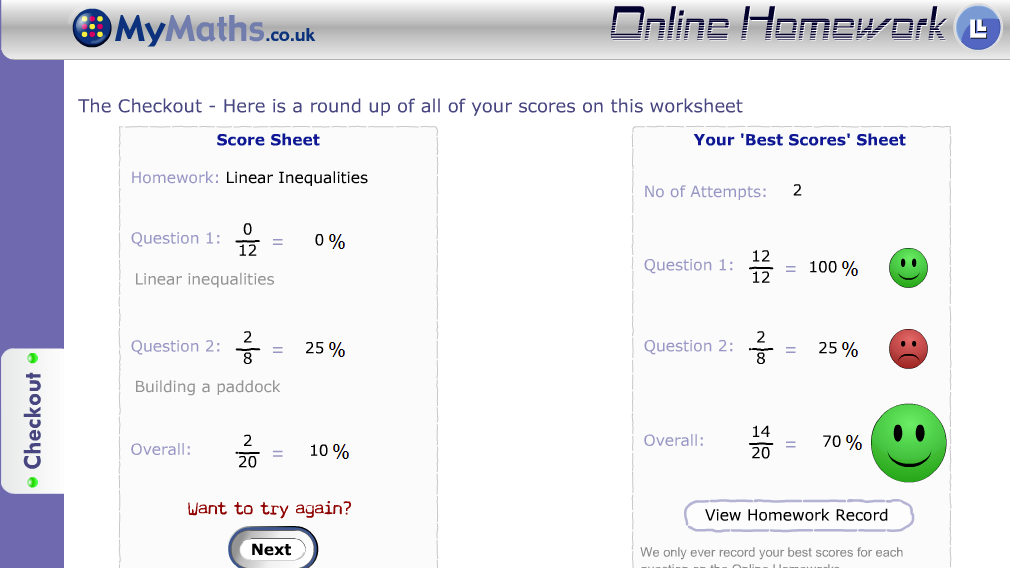
\includegraphics[width=\textwidth]{mymaths}
    \caption{A homework exercise in MyMaths}
  \end{minipage}
\end{figure}
\FloatBarrier

\chapter{Requirements}
\section{Introduction}
As stated in section the main aim of this project is to build an educational game to explain formal logic, mainly through the use of Aristotle's syllogisms. The following requirements are separated into functional and nonfunctional requirements. Functional requirements are concerned with how the game should behave in particular situations with relation to the game's functionality. 
Non-functional requirements place constraints on how the game's functions will complete their tasks, often applying not just to individual functions of the system as a whole

\section{Sources}
\subsection{Literature Review}
The main source of requirements has been drawn from the work in the literature survey. The work carried out that looked into why educational games were so effective allow requirements to be drawn up that ensure the same level of effectiveness when creating this game. Areas such as accessibility, motivation and feedback were extensively researched and the findings have been used to influence these requirements. The discussion of existing serious games and in particular their advantages and disadvantages also provide a source to draw upon.
 \section{Functional}
   \begin{enumerate}[label*=\arabic*]
   
   
   
   
            \item \textbf{The game must scale dynamically to the screen resolution.}\\
It is important when supporting devices of different sizes and screen resolutions that the experience remains consistent across them. In the context of the game this relates to the need for the user interface to scale appropriately, font and font sizes being readable across an array of devices and generally no distortion of images.

            \item \textbf{The game must have multiple levels.}\\
This allows the game to progress in difficulty, allowing the player to begin with the basics and work towards learning more advanced aspects syllogisms and logic.

            \item \textbf{The game must be playable using only the mouse.}\\
As the game is a simple puzzle game there is no benefit to allowing the user to play with the keyboard in addition to the mouse. By allowing only the mouse to used to play the game it will also make it compatible with devices that do not have a keyboard.

 \item \textbf{The game should be playable on tablets and mobile phones.}\\
By allowing the user to interact with the game using only the mouse (finger if on a touchscreen device) and requiring no use of the keyboard it will allow the game to be played across all devices. This aids accessibility as players may not have access to a traditional PC or many want to use a touchscreen device.	


 \item \textbf{The game must feature a tutorial when introducing new concepts.}\\
A tutorial is crucial to explain the premise and controls of the game. With the focus being on the educational aspect of the game it is important to make interacting with the game and getting to grips with the controls as simple and painless as possible.
	 
	  \item \textbf{The game shall have a leaderboard ranking users.}\\
A leaderboard showing how the user performed compared to other people who played the game will increase engagements levels. The leaderboard will rank players based on time taken to complete the game as well as acting as a summative assessment informing the user how well they did. 



 \item \textbf{The game must successfully recognise when the player has completed a level.}\\
The game must be able to accept any valid answer from the user. By not recognising potential end game scenarios it could confuse the user into thinking they are incorrect which would lead to reduced engagement with the game and confusion over what was wrong.	 	

	  \item \textbf{The user shall be able to go backwards and forwards through the tutorials.}\\
The tutorials will be a crucial aspect of the game, with nearly all the new content and information being delivered through them. It is therefore important that the user can navigate backwards and forwards through the instructions in case they need to go over a certain piece of information for a second time.
            
            	  \item \textbf{The system shall track time taken to complete each level and moves made}\\
In order to analyse how effective the game was there will need to be a number of data points recorded. The length of time each level took to complete, along with the number of moves made will be recorded as this allows conclusions to be drawn about how the performance of the user. By combining this data with the initial questionnaire data it will be possible to analyse the effectiveness of the game.
            
            
            	  \item \textbf{The user shall be able to undo and redo actions.}\\
An undo and redo function is crucial for a good user experience especially so in systems involving manipulation of graphics as errors are so easily made. As most desktop and many web applications support this functionality, it would detract the user from the experience if this was not an option. By supporting these functions it allows the user to explore the interface with the freedom to experiment without fear of making an irreversible mistake. 
            
            
            	  \item \textbf{The game should provide visual hints to assist the user.}\\
One of the biggest advantages of using games for education, as mentioned in the literature review, is their ability to provide feedback to the user whilst playing. Therefore it is important to utilise this by providing hints, positive reinforcement and help to the user through on screen graphics during the game.

            	  \item \textbf{The user must be able to save the game.}\\
There should be the functionality for the user to save their place in the game so they can return to it at a later date. This could be useful if the user is interrupted whilst playing the game so they can return to it at a later date and carry on playing from where they left off.
            
                        	  \item \textbf{The system shall easily allow new levels to be added.}\\
With there being 256 syllogisms, although just 24 logically valid, it is important to develop a way to easily add new levels to the game. This is important for both the development of the game as it will allow to easily add new levels and speed up the development phase. This is important as it will allow levels to be added very quickly during the development Also, if the mechanism used to add new levels is simple enough it could be possible for users to create their own levels adding another dimension to the game.

            
            
        \end{enumerate}
        
         \section{Non-functional}
   \begin{enumerate}[label*=\arabic*]
            \item \textbf{It must be possible to play the game on all major browsers.}\\
            This requirement is imperative as accessibility is one of the reasons behind building a web based game. It is important to have a consistent experience across all browsers to not detract from the experience of playing the game. The browsers targeted will be current list of browsers as maintained by W3Schools. As most minor browsers are built using the same underlying technology as one of the major ones, provided it works on all of the most popular ones there is a very high chance it will work on the minor ones.    
            
            
             \item \textbf{There must be an initial prototype of the game.
}\\
            Following an agile methodology when carrying out software development requires the application to be built incrementally. A minimum viable product should be built and then features incrementally added. By using this approach when developing the game it will mean that there will be an initial prototype that can be used to gather user feedback. Supervisor feedback can also be given to steer the project in the right direction and anything that needs to be added can be picked up at the development phase before full user testing takes place.
            
            
                         \item \textbf{The game must have an elegant user interface.}\\
It is important to not crowd the users with an excessive number of buttons and options in the game. As no keyboard controls will be used, the challenge will be to provide a way to operate all controls of the game efficiently.
            
                        
                         \item \textbf{The game must appear smooth to the user.}\\
When creating applications that a user interacts with it is important to consider the delays taken between the user interacting with the system to the result being shown on screen. For the game to appear to run without delay, it would ideally react to user input within 100ms. \citep{nielsen1994usability} explains a delay of less than 100ms will give the user the feeling of the system reacting instantaneously. A delay of longer than 100ms can lead to the user losing their focus on the task and can require feedback from the system informing the user of the delay. User experience guidelines published by Google delve further into this area and say that 16ms is the maximum response time for animations. As this system is a game, that will heavily feature animations, this is important to consider.
             
                                      \item \textbf{The navigation toolbar must remain consistent throughout the game.
                                      }\\
It is important that the navigation bar does not change location throughout the game as it could confuse the user. It is also important that all the options available are present for every level. For example if some levels do not have an undo option it could lead to confusion for the user.

                                      \item \textbf{The game must motivate the user to learn about syllogisms
}\\
The game must engage with the user and maintain their attention. It's important to create an environment where the user wants to be playing the game so that the intrinsic desire to play through the levels is strong. It is therefore important to balance the educational aspect with enjoyment and getting the difficulty of the levels correct as to not demotivate the user.
            \end{enumerate}
            
\chapter{Design}

\section{HTML}
HTML (Hyper Text Markup Language) describes the structure of web pages. The purpose of a web browser is to read and display HTML pages. HTML is only used to define the content of a web page and not how it should be formatted for the end user.
An important part of HTML is the DOM (document object model). When a web page is opened the browser creates a document model of the page to which objects can be added, modified and removed.

\section{CSS}
CSS (Cascading Style Sheets) defines how HTML elements are displayed on a page, essentially allowing formatting to be added such as colour, fonts and layout. It allows web pages to react to different screen sizes and speeds up the development of projects as styles can be applied to groups of HTML elements. 

\section{JavaScript}
Initially the web was made up of sites built using HTML and CSS serving static content. As the web progressed there was a desire from developers to create more interactive websites and to respond to these interactions without needing to make relatively expensive calls to a server. This is where JavaScript, a client side programming language, came in. JavaScript allowed elements in the DOM to be interacted with dynamically resulting in a much richer web experience.

\section{SVG}
SVG (Scalable vector graphics) is a technology that was released in 2001. 
It uses XML to define vector images that are retained by the browser. SVG is used with the <svg> tag and acts similarly to a <div> HTML tag. It acts on a higher level than Canvas, mentioned later, as objects are stored and remembered in the DOM. This means that all objects created are remembered by the DOM meaning they can be kept track of much easier and natively handle events such as mouse clicks.

\section{Canvas}
Canvas is a technology that was originally designed by Apple in 2004. It was later adopted as a web standard and included as part of HTML5, the current HTML standard introduced in 2014. By adding the <canvas> element to HTML it is possible to draw graphics using JavaScript. Canvas allows for the drawing of immediate mode graphics, meaning that once the pixels have been draw to the screen there is no record of these pixels maintained. In turn this means that any time something on the Canvas changes, everything needs to be redrawn. 

\section{Canvas Libraries}
There are a large number of Canvas libraries out there that aim to simplify many aspects of using Canvas. Fabric.js, Paper.js, Easel.js and Phaser were all looked at with regards to being used in this project. The main features of these libraries include adding support for clicking and dragging objects on the Canvas, simplifying the drawing shapes and assist in animation.
The disadvantage of using these libraries is that they are more focussed on traditional games that rely heavily on animations and not the slower puzzle style that is being developed in this situation. They also abstract away the inner workings of Canvas and can add unnecessary complications to developing what is a reasonably simple game. For this reason it was decided to write the game with no libraries but to just use pure JavaScript.

\section{Game Design}
The overall design of the game is that of a puzzle style with the user working their way through multiple levels of increasing difficulty. The basic mechanics require the user to drag and drop items, usually numbers and shapes, into Venn Diagrams. Each level usually has a statement or fact that must be represented diagrammatically through the correct placement of objects in the venn diagrams.

\section{User Interface}
The goal of the user interface was to be as simple as it possibly could be whilst still allowing all the required functionality to be added. The approach taken with the design was to keep it as clean and minimalist as possible so not distract the player with unnecessary clutter. The relatively small amount of on-screen items also was a benefit when ensuring the game worked well on smaller resolution devices where screen real estate is at a premium. UI mock ups were created that could be shown to users for feedback and acted as a starting point once development began.

\begin{figure}[h]
  \centering
  \begin{minipage}[b]{1\textwidth}
    \includegraphics[width=\textwidth]{EvenNumbersMultiple5Mockup}
    \caption{UI Mockup}
  \end{minipage}
\end{figure}
\FloatBarrier

\section{Control Bar}
There are a number of controls that are needed to be present at all times apart from when the user is going through a tutorial. A control bar that remains consistent both in its placement and options available throughout the game will stop the user from feeling confused and allow them to feel confident when interacting with it. The icons chosen were hugely important as there would be no labelling of them so there functionality would have to be shown purely through their image. The icons chosen are based on Google's Material Design icons. It is hoped that through this choice the icons that have been chosen will be familiar to users and as such their function is obvious.

\begin{figure}[h]
\centering
    \includegraphics[scale=0.5]{NavigationBar}
    \caption{Control Bar}
    \label{fig:floodFillBad}
\end{figure}
\FloatBarrier

\section{Tutorial Design}
There will be a number of tutorials throughout the game so it is important to have a clear and consistent structure to them throughout. This will let the user know when a tutorial is happening so they can pay close attention as it will mean new ideas are about to be introduced. The general structure to the templates involves instructions being displayed on the screen with arrows being drawn to point to the relevant area. There are also forwards and backwards buttons at either side of the screen for the user to navigate their way through the tutorials. 

\section{Level Design}
It was very important to design the levels with the correct level of difficulty. If the game started off too hard it would demotivate the player and stop them from wanting to play. Conversely, if the game was too easy and did not introduce harder concepts as the levels progressed their would be no challenge to keep the user interested.

The general idea was to initially have very simple levels that introduced the mechanisms and controls for how the game worked. It also acted as a refreshed on some basic set theory ideas such as empty sets. 

From there a level was added that discussed with a simple example how venn diagrams worked. This would most likely have been a refresher as opposed to new content for most users as venn diagrams are a commonly taught way to represent sets in UK schools.

In response to early stage user testing a level was also added that taught the user about empty sets. This was initially an oversight and it was not until users tried to complete the game it became clear that the concept and understanding of empty sets was less prevalent than first thought.

After this there are a number of syllogism levels. The first one is structured with a very tutorial heavy focus. Every step of process from dragging the words into the correct circles to completing the syllogism line by line is aided by the tutorial system guiding the user through the process. After the tutorial the syllogisms get progressively harder with particular syllogisms added, involving the word "some".

As an addition to the game, once the syllogism levels are completed there are a few levels that cover set theory. They aim to teach the basics such as the union and intersection of sets as well as the distributive and associative laws. 



\chapter{Implementation}

\section{Undo and Redo}
As Canvas does not maintain any record of drawings on the canvas there is no in-built functionality that allows a user to undo or redo an action. In order to achieve this, it must be implemented manually.

There are two ways this can be done; storing everything that is drawn on the canvas in a stack or by capturing the screen as a image and using that image to redraw the canvas. Both options were investigated to see which was the best.

Tests were ran on the execution time of both saving the entire canvas image and using a data structure to store the game state. Saving the entire canvas took 16 milliseconds compared to just 0.1 milliseconds to push the GameState to the stack, 160 times faster. Whilst 16 milliseconds is an acceptable amount of time for an action to take and in isolation does not have an effect on user experience, in combination with other functions that must run on an undo or redo this begins to affect performance. Also as the number of moves increases the number of full canvas images must be stored increases which can lead to memory issues on certain browsers. Another issue with using the image method is that whilst the canvas will revert to its previous image, the underlying state of the game will be incorrect. This is not an issue when using a stack as the location of all the users clicks are stored so the game state is reflected to show this.

The best option was every time a move is made, the current state of all the objects is stored in a data structure and pushed to the stack. When the user presses the undo button, the top object in the stack is popped and everything is redrawn. Despite there being many different objects on the Canvas, the only ones that the user can interact with is the movable text, which can be dragged around, and filling in the circles. Therefore the current state of the game can be represented as:

\begin{lstlisting}
var GameState = function (movableTextArray, clickedInArray) {
   this.movableTextArray = movableTextArray;
   this.clickedInArray = clickedInArray;
};
\end{lstlisting}


\section{Clicking on items}
As previously mentioned, Canvas uses immediate mode graphics to draw pixels to the screen meaning that once they've been draw Canvas forgets about them. So this means that recognising when a user clicks on an object is not something that is natively supported by Canvas and must be implemented manually. 
For example, take the level where there are 3 dogs that need to be dragged into the circle. First once the levels loads an array is created which holds the three images as well as properties such as the location of the image and its width and height.
\begin{lstlisting}[language=json]
[
  {
    "id": "dog1",
    "width": 51,
    "height": 51,
    "y": 857,
    "x": 294,
  },
  {
    "id": "dog2",
    "width": 51,
    "height": 51,
    "y": 857,
    "x": 934,
  }
]
\end{lstlisting}

Then, any time the user clicks on the screen a check if done to see if that mouse click is inside one of the images in the array.
This is done by looping through the array and checking to see if the x and y of the mouse click fall inside the bounding rectangle of the image and then return the index of the image that has been clicked in.

\begin{lstlisting}[language=JavaScript]
function imageClickedOn(x, y, movableTextArray) {
    for (var i = 0; i < movableTextArray.length; i++) {
        if (x >= movableTextArray[i].x &&
            x <= movableTextArray[i].x + movableTextArray[i].width &&
            y >= movableTextArray[i].y &&
            y <= movableTextArray[i].y + movableTextArray[i].height) {
            return i;
        }
    }
    return -1;
}
\end{lstlisting}


\section{Dragging items}
Dragging images and text around the screen is the core of the game, and another feature that Canvas does not provide so again must be implemented manually. 
First when the user clicks on an image the mouse click event is triggered and all the images are checked to see which one was clicked on, as detailed above. The clicked on image array index is stored as well as a drag offset, which contains the exact location on the image that was actually clicked.
When the user then moves their mouse the mouse move event is fired. This checks to see if the drag boolean is true and if it is updates the x and y location of the image to the new mouse location minus the drag offset that was stored. This reason that a drag offset must be stored is that without it the dragging would always take place from the x,y coordinates of the image which in Canvas' case is the top left. So no matter where the user clicked on an imagine they would experience dragging from the top left. Every time the mouse is moved until it is released the x and y get updated and each time that happens everything on the screen needs to be redrawn. 
There are three ways to do this, setInterval, setTimeout and requestAnimationFrame. Initially, setTimeout was used as it is supported by all browsers. It works by calling a function every specified number of milliseconds. In the table below 1000/60 is used as the interval at which to call the function as this represents 60 frames per second. However, there was often a noticeable amount of delay when lots of intensive tasks were being animated, especially on lower powered devices such as mobile phones.

Therefore, another solution needed to be found. requestAnimationFrame is an API provided by browsers that handle the drawing of animations for both Canvas and DOM-based changes. This allows the browser to perform a number of optimisations such as preventing unnecessary redraws, call pool multiple animations into a single redraw cycle and prevent animations from running on tabs that are not currently open. As table shows, requestAnimationFrame is considerably faster than the other two options. Unfortunately, not all browsers support requestAnimationFrame meaning that a polyfill is needed that allows the browser to fall back to setInterval should requestAnimationFrame not be supported.

\begin{lstlisting}
window.requestAnimFrame = (function(){
  return  window.requestAnimationFrame       ||
          window.webkitRequestAnimationFrame ||
          window.mozRequestAnimationFrame    ||
          function( callback ){
            window.setTimeout(callback, 1000 / 60);
          };
})();
\end{lstlisting}


\begin{table}[ht]
\centering
\begin{adjustbox}{width=1\textwidth}
\small
\begin{tabular}{ c | c }
  \hline
 Function & Operations per second \\ \hline 
    setInterval & 39 \\
    setTimeout & 43 \\
    requestAnimationFrame & 61 \\
   \hline
\end{tabular}
\end{adjustbox}
\caption{Best way to animate test} 
\end{table} 

\section{Saving the game}
One requirement was that it must be possible for the game to be saved so that the user could return at a later date and carry on playing from where they left off. There are a number of possible solutions for saving the state of a game in the browser.

Previously to achieve this any storage of data would have to have been done through the use of cookies. A cookie is a way to store a small amount of data, up to a maximum of 4kb, in a text file on a user's computer which expire after a certain amount of time.

With the introduction of HTML5 a new method for storing data in the browser was added, localStorage. This new mechanism allows 5MB of data to be stored locally on the browser and is then accessible through any JavaScript that is running on the same domain. It has been implemented here by saving the user's progression after every level that is completed.

So in order to save the game an object is created that holds the current state of the game. This contains both the current level number and the name of the user. Every time a level is completed the object is updated with the new level number and that object is then saved. There is no need to remove the old object as the localStorage API silently overwrites the existing object if the key already exists.


\begin{lstlisting}[language=JavaScript]
\\save object
localStorage.setItem('gameObject', JSON.stringify(game));
\end{lstlisting}

The next time the user returns to the web page this saved object can be retrieved.
\begin{lstlisting}[language=JavaScript]
var retrievedObject = JSON.parse(localStorage.getItem('gameObject'));
\end{lstlisting}

The option to resume play is presented to the user through a 'continue' button on the home page. The continue button is initially hidden and by checking that the object retrieved from local storage is not null it can be made visible.

\begin{lstlisting}[language=JavaScript]
if (retrievedObject != null) {
   $("#continueButton").visible();
}
\end{lstlisting}

\section{Saving data to database}
One of the requirements was for a leaderboard that provides users with the option to enter their name and be able to see how they rank alongside other people who have played the game. This also doubles up as a way to gain an extra layer on analysis being able to take a deeper look at how long levels took and the number of moves that were made. 

Initially a REST (REpresentational State Transfer) service was to be created to handle the transport of data. REST uses the HTTP protocol to manipulate data through requests such as GET, which returns data from a datbase and POST which persists data in a database. The REST service would act act as the intermediary between the client side and the database.

\begin{figure}[h]
  \centering
  \begin{minipage}[b]{1\textwidth}
    \includegraphics[width=\textwidth]{REST}
    \caption{Basic REST service architecture}
  \end{minipage}
\end{figure}
\FloatBarrier

This would require writing REST endpoints to handle such data, using a language such as Node.js, a variant of JavaScript designed to run server side. The problem with this solution is that it requires not only the writing of a REST service but also setting up a database and acquiring a server to host both of these on. This is overkill for the needs of this project as no sensitive data is being stored, only a few columns of data are needed and speed and number of possible connections that can be sustained are of no concern.
 
Therefore, for this project Google Sheets is being used as a cloud based database. Google sheets is a web based spreadsheet application, very similar in functionality and appearance to Microsoft Excel. Whilst Google Sheets does not offer the same depth of functionality as desktop based solutions it is perfect for storing a relatively small amount of data with no significant analysis needing to be performed.

Google Sheets does not explicitly support the functionality of using it to act as a database, and as such there are a number of workarounds that must be carried out to make this possible.
Google Scripts is a cloud based scripting platform operated by Google that allows JavaScript code to be written that can interact with other Google products, such as Sheets. By using this, it is possible to create what is equivalent to a REST endpoint all hosted within Google's platform. 
Data can then be posted to this Google Script URL from the game's code that will handle the data and insert it into a Google Sheet.

An object is created that stores all the data that is to be posted, in this case the time and moves taken to complete each level. This object is then serialised for use in a URL query string. This serialised object is then sent to the Google Scripts endpoint via an AJAX request. AJAX (Asynchronous JavaScript and XML) allows client side code to communicate with a web server without needing to reload the page. The asynchronous nature means that the client side code will continue to execute without waiting for a reply, returning only once a reply has been received. This prevents the user from having to wait for the request to be returned.


\begin{lstlisting}[language=JavaScript]
request = $.ajax({
   url: "https://script.google.com/macros/s/AKfycbxVGVxoQxNFK7_nxKfglL8yLNUmdPwP2e9j8IMO6JY5wzLEdSE/exec",
   type: "post",
   data: serializedData
});
\end{lstlisting}

\section{Reading from database}
Saving data to the database is just one part of the problem, in order to have a functioning leaderboard system it must also be possible to read that data back.

The JavaScript library Sheetrock\.js allows Google Sheets to be interacted with as if they are a traditional database through the use of SQL-like statements.
For example, in traditional SQL the query to get the 5 fastest play though times would be:

\begin{lstlisting}[
           language=SQL,
           showspaces=false,
           basicstyle=\ttfamily,
           commentstyle=\color{gray}
        ]
SELECT TOP 5 time_taken, moves_made, levels_skipped FROM leaderboard ORDER BY time_taken ASC;
\end{lstlisting}

In Sheetrock.js a similar syntax is used:

\begin{lstlisting}[language=JavaScript]
$('#spreadsheet').sheetrock({
   url: mySpreadsheet,
   query: "select B,W,X order by X asc",
   fetchSize: 5
});
\end{lstlisting}

Which get the data from the Google Sheet and fills into the HTML table element with the ID 'spreadsheet'.

\section{Working across multiple platforms}
As this game is designed to run across browsers and mobile devices, it is important that the experience is consistent across all potential screen resolutions. The way that has been chosen to do this is everything drawn on the canvas is relative to the height and width of the screen. 
For example, when creating the circles to represent the venn diagram the following is done:

\begin{lstlisting}[language=JavaScript]
if (circlesNeeded === 3) {
    //split the screen in to 4 vertical segments
    var segments = canvasHeight / 4;
    //set the radius of each circle
    var radius = segments / 2 * 1.25;

    var overlap = radius / 2;
    circlesArray.push(new Circle((canvasWidth / 2), (segments + (segments * 2)) / 2 + (segments / 6), radius));
    circlesArray.push(new Circle((canvasWidth / 2) - overlap, (segments * 2 + (segments * 3)) / 2 - (segments / 6), radius));
    circlesArray.push(new Circle((canvasWidth / 2) + overlap, (segments * 2 + (segments * 3)) / 2 - (segments / 6), radius));

\end{lstlisting}

This allows the user interface to look exactly the same across all screen resolutions. 
Canvas is supported by the all the major desktop browsers but still has a number of bugs present on Internet Explorer and FireFox. It is also supported by Android and iOS browsers but some work must be done to actually make it work for touchscreen devices. Touch events must be defined to handle the user touching the screen and dragging their finger along the screen. When using jQuery, the user touching the screen is handled by:


\begin{lstlisting}[language=JavaScript]
$(window).bind('touchstart', function (jQueryEvent)

\end{lstlisting}

\section{Floodfill}
In order to allow the user to fill in sections of the circles to represent ideas such as the empty set, a flood fill algorithm is needed. A flood fill behaves in the same way as a paint bucket tool in many image editing programs, filling an area of connected pixels with the same colour. There are a number of different algorithms that can achieve this, with recursive and stack based solutions the two most popular. The issue with recursive solutions is that given a complex image there can be a huge number of recursive calls made, potentially causing stack overflow. 
Therefore, the implementation chosen was to use a stack and a while loop.

\begin{itemize}
   \item  First the x,y location of the mouse click is added to a pixelStack
   \item While there are elements in pixel stack
   \begin{itemize}
     \item  Pop top value from pixel stack and assign to x and y
\item  Travel upwards one pixel at a time until boundary hit or different colour pixel is found
\item  Now travel downwards one pixel at a time until boundary hit or different colour pixel is found. This time colouring pixels with new colour as we go.

\item  Now check pixel to left to see if it needs colouring
\item  If it does need colouring add pixel to stack and set a boolean goLeft to true

\item  Now check pixel to right to see if it needs colouring

\item  If it does need colouring add pixel to stack and set a boolean goRight to true

\item  Move down 1 pixel

\item  Look left and right

     \begin{itemize}
       \item  If left or right needs colouring but respective boolean set to true then do not add to stack
\item Else if left or right needs colouring but respective boolean set to false then add to stack
     \end{itemize}
     \item Keep moving downwards until boundary or different colour pixel is hit
\item One column is now filled in, but the stack still has pixels in it so go back to start, pop next pixel and run through again.

   \end{itemize}
 \end{itemize}
	

This algorithm works well but unfortunately has a few problems. Figure \ref{fig:floodFillBad} shows that when using this solution it is not possible to get a \textit{clean} flood fill. This means that the colour black is not filled all the way to the edge and there is a jagged outline due the inherent problem that flood fill algorithms have with anti-aliased edges.

\begin{figure}[h]
\centering
    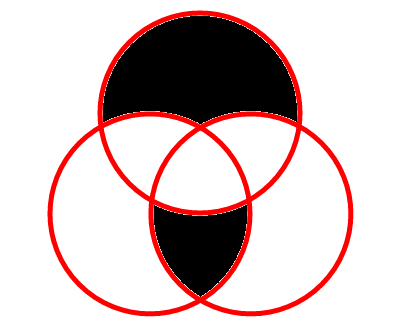
\includegraphics[scale=0.5]{floodFillBad}
    \caption{Stack based floodfill algorithm}
    \label{fig:floodFillBad}
\end{figure}
\FloatBarrier

	A solution was found by using the library FloodFill2D which implements a more sophisticated floodfill algorithm to specifically deal with the anti-aliasing issue. This library allows a tolerance fade to be set that allows a soft edge to be created at boundaries. However, even that did not completely resolve the problem. In order to get a completely clean appearance to a floodfill more needed to be done. The solution was to create a new Canvas element that sat on top of the one currently being used to draw the circles. This new layer would be used to draw identical circles at a thicket width that would cover up the rough edges on the inner perimeter of the circle. This would not effect the floodfill as the algorithm only floodfills on one Canvas so has no knowledge of these new, wider diameter circles.

\section{Recognising when level is complete}
The location of each text item is found:
\begin{lstlisting}[language=JavaScript]
    var middle = whichCircleIsPremiseIn(level.movableTextArray[0]);
    var predicate = whichCircleIsPremiseIn(level.movableTextArray[1]);
    var subject = whichCircleIsPremiseIn(level.movableTextArray[2]);
\end{lstlisting}

The location of each intersection is then also stored based on the location of the middle, subject and predicate.
The correct answer is for each level is stored in the JSON as so:
\begin{lstlisting}[language=json]
"correctSyllogism": {
      "subject": true,
      "middleSubjectIntersection": true,
      "subjectPredicateIntersection": true,
      "middlePredicateIntersection": false,
      "middleSubjectPredicateIntersection": false,
      "predicate": false,
      "middle": true
}
\end{lstlisting}

A new object is created with the same structure as the correct syllogism object.
Every time the user clicks in a segment of the circles, which fills it black, the location of the click is stored. This is array of user clicks is used in conjunction with the location of the text to set each location to true or false. From there the correctSyllogism object stored in the game level JSON can be compared with the new object that has been built up by checking the location of the terms to see if they are the same. If both objects are equal then it means that the level has been completed.

\section{Visual Feedback}
As previously mentioned one of the big advantages to using games to educate is that they can provide the user with immediate feedback. There are a number of ways that this have been achieved in this game. When placing items in the circle, the game checks to perform that the placement is valid and if so highlights the circle in green. This immediately shows the user that they have made a correct move.  This is achieved by checking each premise is inside the same circle as another premise.

\begin{lstlisting}[language=JavaScript]
function checkPremiseAllInTheirOwnCircle() {
    var middle = whichCircleIsPremiseIn(level.movableTextArray[0]);
    var predicate = whichCircleIsPremiseIn(level.movableTextArray[1]);
    var subject = whichCircleIsPremiseIn(level.movableTextArray[2]);

    if (middle == null || predicate == null || subject == null) {
        return false
    } else {
        return !(middle.equals(predicate) || middle.equals(subject) || predicate.equals(subject));

    }
}
\end{lstlisting}

\begin{figure}[!h]
  \centering
  \begin{minipage}[b]{0.4\textwidth}
    \includegraphics[width=\textwidth]{GreenHighlightCorrectPlacement}
    \caption{Correct Placement}
  \end{minipage}
  \hfill
  \begin{minipage}[b]{0.4\textwidth}
    \includegraphics[width=\textwidth]{GreenHighlightIncorrectPlacement}
    \caption{Branching Temporal Logic}
  \end{minipage}
\end{figure}
\FloatBarrier

When completing the syllogism levels there are 3 statements that must be made true; the major premise, the minor premise and the conclusion. When the user makes any of these three true the words font colour of the sentence changes to green.


\begin{figure}[h]
\centering
    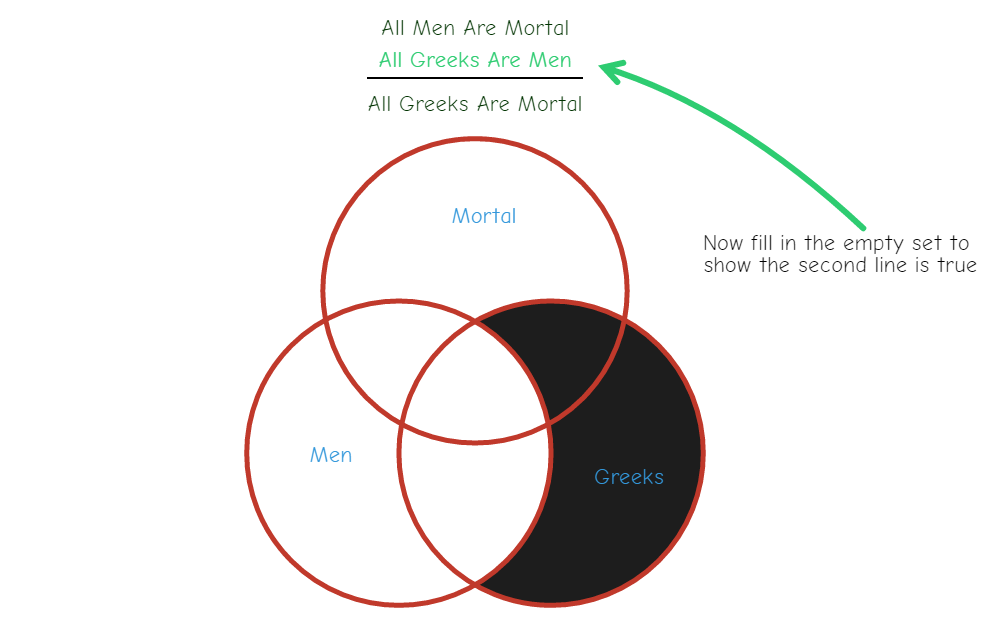
\includegraphics[scale=0.5]{PremiseHighlight}
    \caption{Premise Highlighting}
    \label{fig:floodFillBad}
\end{figure}
\FloatBarrier


\bibliographystyle{plainnat}
\bibliography{bibliography} 

\end{document}